\documentclass[a4paper, 12pt]{article}

% osnovni paketi za jezik in kodiranje znakov
\usepackage[slovene]{babel} 
\usepackage[utf8]{inputenc}
\usepackage[T1]{fontenc}
\usepackage{lmodern}

% dodatni paketi
\usepackage{amsmath, amssymb, amsthm}
% \usepackage[font=small, center]{caption}
\usepackage[hidelinks]{hyperref}
\usepackage{graphicx}
\usepackage{wrapfig}
\usepackage{float}     
\usepackage{geometry}
\usepackage[table]{xcolor} % http://ctan.org/pkg/xcolor
\usepackage{biblatex}
\addbibresource{literatura.bib}


\begin{document}

\begin{titlepage}
    \begin{center}
        \large
        Fakulteta za matematiko in fiziko\\
        Oddelek za matematiko \\
        \vspace{6cm}
        \Huge
        \textbf{Vizualizacija Kakeya-množice} \\
        \vspace{6cm}
        \large
        Terezija Krečič\\
        Pedagoška matematika, 5. letnik\\
        \vspace{1cm}
        Predmet: Matematika z računalnikom \\
        Mentor: Sergio Cabello\\
        \vspace{2cm}
        Ljubljana, 21. 5. 2024
    \end{center}
\end{titlepage}

\newpage


%%%%%%%%%%%%%%%%%%%%%%%%%%%%%%%%%%%%%%%%%%%%%%%%%%%%%%%%%%%%%%%%%

\section*{Uvod}

V tej projektni nalogi je bil cilj vizualizirati Kakeya-množico s pomočjo programa \href{https://ipe.otfried.org/}{Ipe}. Najprej sem morala sploh predelati problem, ki ga je zastavil Kakeya več kot sto let nazaj, poleg tega pa se še spoznati z novo programsko opremo.

Poročilo sem zapisala kar v obliki članka in vizualizacijo vključila kot spremne slike ob besedilu. Vse slike sem ustvarila sama s pomočjo omenjenega orodja Ipe (le slika~\ref{primeri} je narejena v Geogebri, saj deltoide v Ipe nisem znala vizualizirati).

Poročilo je izhaja iz Besicovitchevega članka~\cite{Besicovitch}, vendar sem nekaj delov poenostavila in predelala, saj sem se poskusila čimbolj izogniti upeljevanju novih oznak, ki bi bralca zmedle. Tudi pri poljubno majhni ploščini Pálovega spoja nisem uvedla poljubno majhnega kota $ \epsilon $ in z njim zapisala formulo za ploščino spoja (ki je ravno tako poljubno majhen v odvisnosti od $ \epsilon $), temveč sem idejo zapisala le z besedami.

V članku bo najprej predstavljeno zastavljeno vprašanje, ki ga rešujemo, nato pa še en način generiranja take množice, ki ustreza pogoju iz vprašanja in nanj tudi odgovori. Menim, da je članek dovolj poenostavljen, hkrati pa še vedno strokoven, da bi ga razumel tudi marsikateri srednješolec.

\newpage

%%%%%%%%%%%%%%%%%%%%%%%%%%%%%%%%%%%%%%%%%%%%%%%%%%%%%%%%%%%%%%%%%

\section*{Kakeyev problem igle}

Japonski matematik Sōichi Kakeya je leta 1917 zastavil naslednje vprašanje, ki se ga je v kasnejšem času prijelo ime ``\emph{Kakeyev problem igle}''\footnote{orig. \emph{the Kakeya needle problem}, op. prev.}: \textbf{Kolikšna je lahko najmanjša ploščina območja, znotraj katerega se daljica dolžine 1 zvezno obrne za 360°?}

\noindent Poglejmo si tri primere geometrijskih likov, ki ustrezajo pogoju iz vprašanja:

\begin{enumerate}
    \item krog s premerom 1 $ \rightarrow $ ploščina $ = \frac{\pi}{4} \doteq 0{,}79 $
    \item enakostranični trikotnik z višino 1 $ \rightarrow $ ploščina $ = \frac{1}{\sqrt{3}} \doteq 0{,}58 $
    \item deltoida\footnote{za konstrukcijo deltoide gl.~\cite{deltoida}, za animacijo obračanja igle znotraj nje pa~\cite{kakeya_wiki}}, včrtana v krog s premerom $ \frac{2}{3} $ $ \rightarrow $ ploščina $ = \frac{\pi}{8} \doteq 0{,}39 $
\end{enumerate}

\begin{figure}[h!]
    \centering
    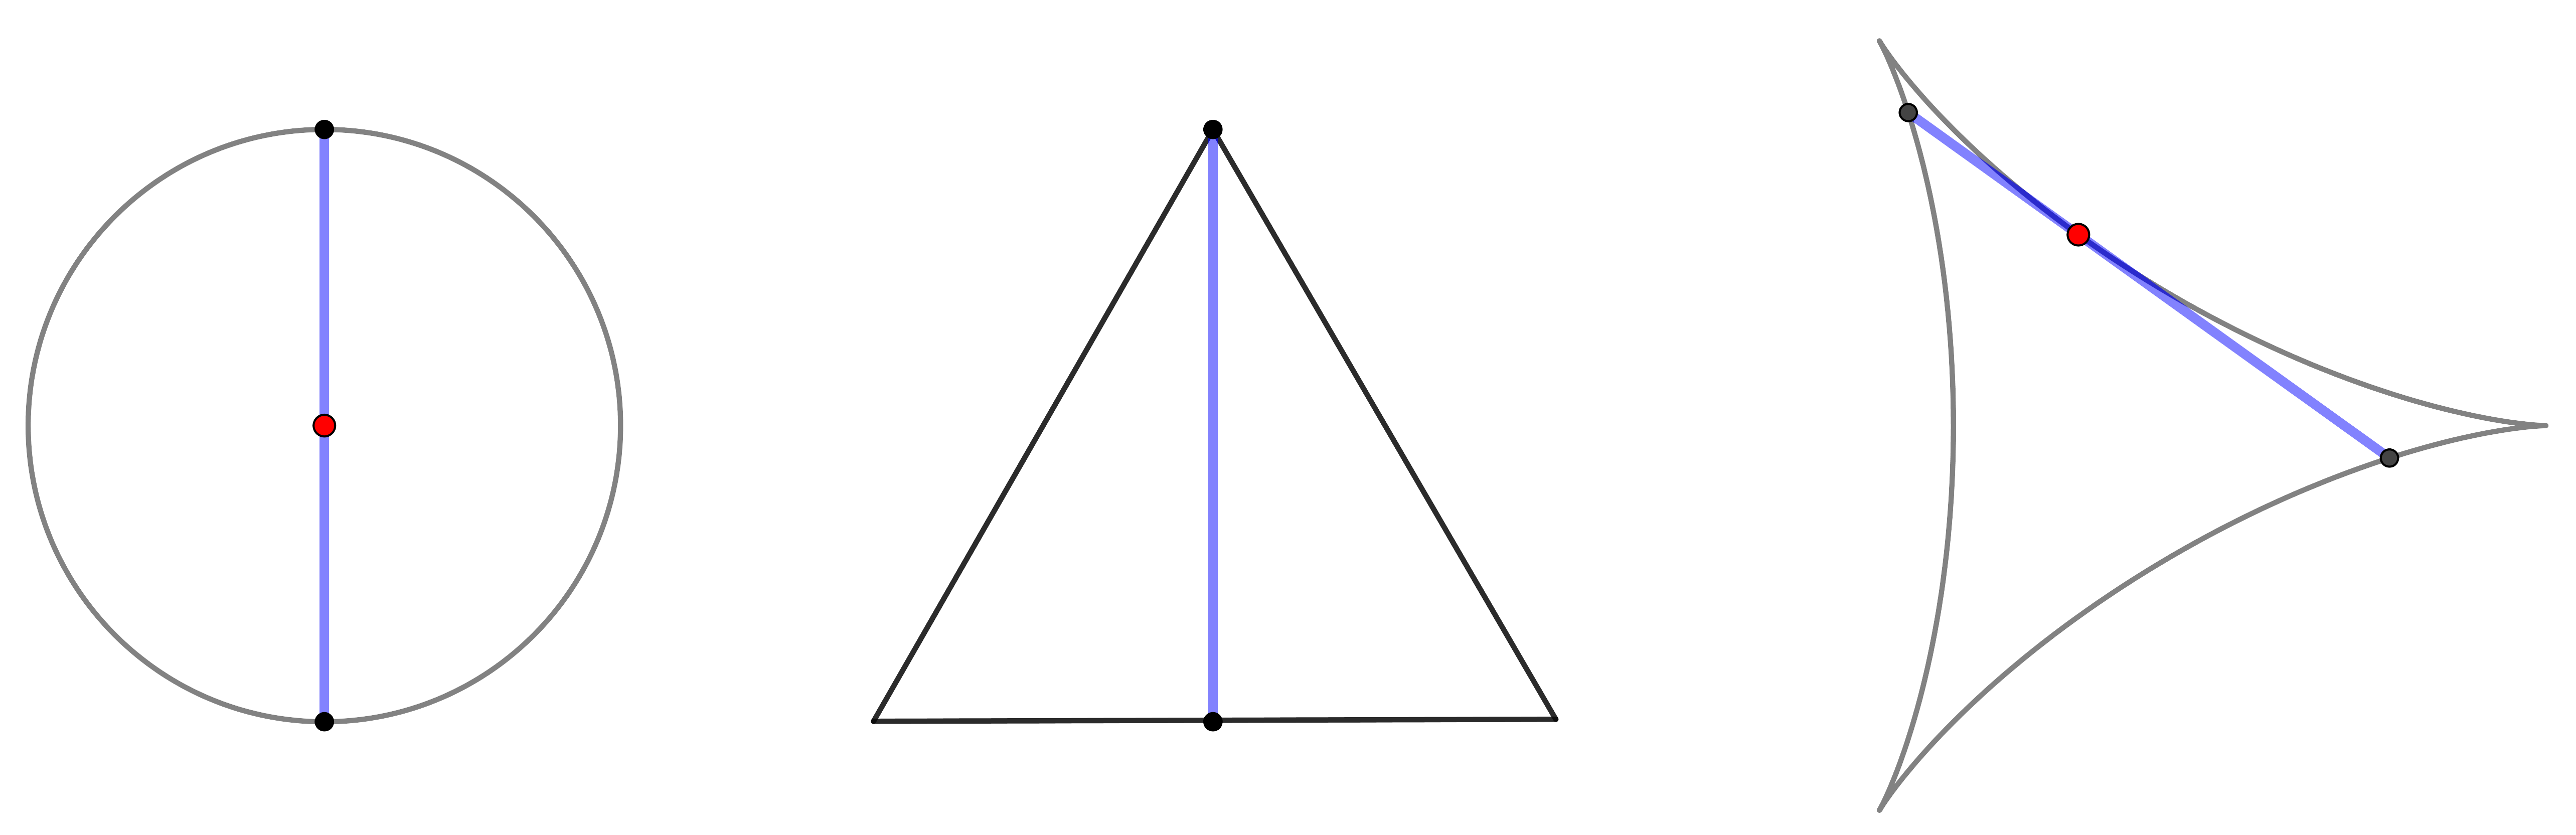
\includegraphics[width=0.8\textwidth]{geogebra_slike/prevelike_ploscine.png}
    \caption{Primeri, ki ustrezajo pogoju.}
    \label{primeri}
\end{figure}

Nekaj časa so verjeli, da je deltoida odgovor na vprašanje Kakeye, vendar je ruski matematik Abram Besicovitch uspel dokazati, da \textbf{spodnja meja za iskano ploščino \emph{ne} obstaja}. K enostavni konstrukciji primera takega lika je pripomogel nemški matematik Oskar Perron, pomemben del pa je prispeval tudi madžarsko-danski matematik Gyula Pál.

%%%%%%%%%%%%%%%%%%%%%%%%%%%%%%%%%%%%%%%%%%%%%%%%%%%%%%%%%%%%%%%%%

\section*{Ideja za konstrukcijo}

Vzemimo enakokraki pravokotni trikotnik s katetama dolžine 2. Če v središče hipotenuze postavimo en konec enotske daljice, njen drugi konec opiše kot 180°, pri čemer daljica ves čas ostane znotraj lika. Nato jo po hipotenuzi potisnemo do začetne pozicije in še enkrat zavrtimo -- tako se daljica res zavrti za 360°. Trikotnik sicer ustreza pogoju iz vprašanja, vendar je njegova ploščina enaka 2 in večja od vseh treh zgornjih primerov.

Sedaj ga razdelimo na pol, kot kaže slika~\ref{trikotnik_razdelitev}, ter vsakega izmed delov (ki sta še vedno enakokraka pravokotna trikotnika, imenujmo ju ``\emph{osnovna trikotnika}'') še dodatno razdelimo na $ n $ manjših trikotnikov (imenujmo jih ``\emph{podtrikotniki}'') z osnovnico dolžine $ \frac{2}{n} $ in višino 1. Enotska daljica se tako obrne za 180°, ko se v enem krajišču zasuče čez vrh vsakega izmed podtrikotnikov in prehaja med njimi preko skupnih stranic.

\begin{figure}[h!]
    \centering
    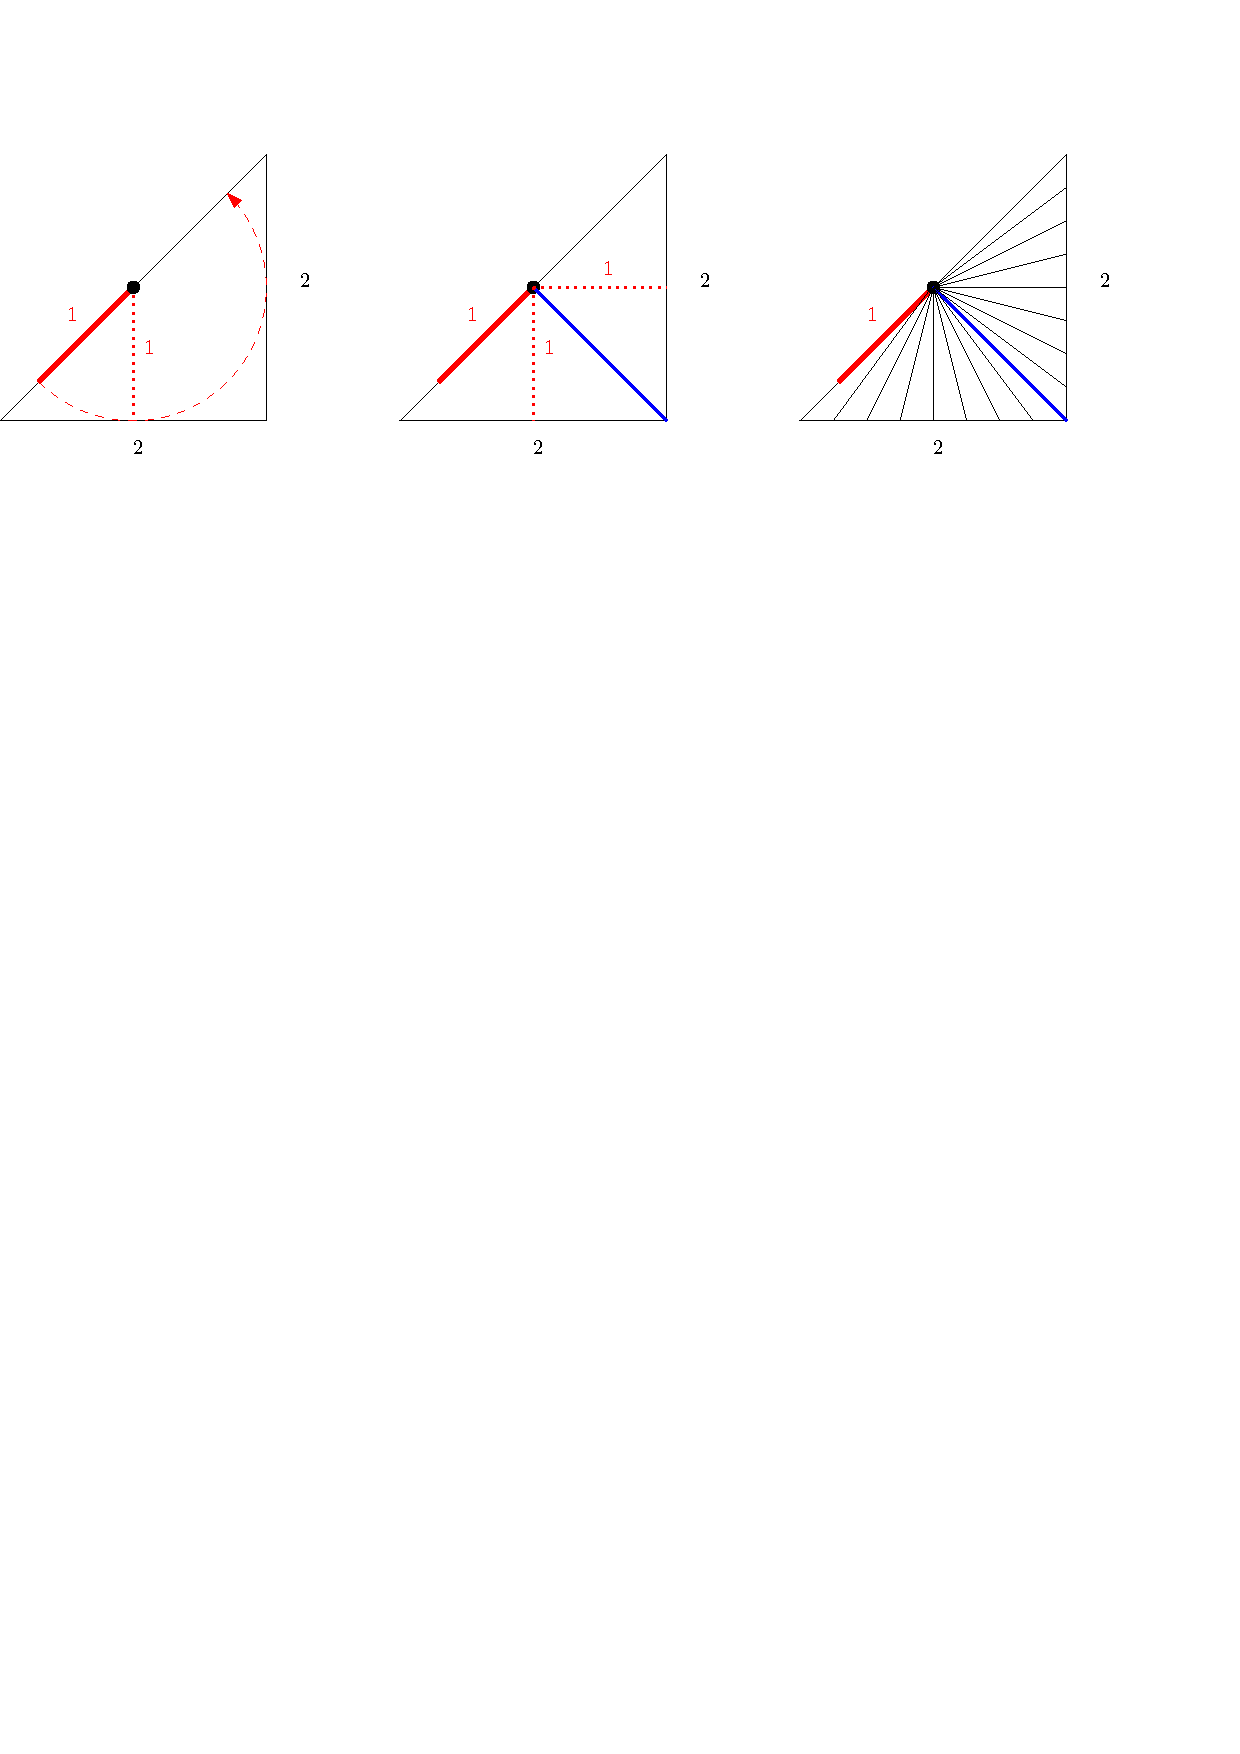
\includegraphics[width=\textwidth]{ipe_slike/trikotnik_razdelitev.pdf}
    \caption{Generiranje $ 2n $ podtrikotnikov z višino 1.}
    \label{trikotnik_razdelitev}
\end{figure}

\textbf{Ideja je, da teh $ 2n $ trikotnikov tako vzporedno premaknemo, da skupno prekritje tvori lik s poljubno majhno ploščino, ko $ n \to \infty $.}

Takoj opazimo, da se s translacijo podtrikotnikov prekine zvezen prehod enotske daljice iz enega podtrikotnika na drugega. Na sliki~\ref{preskok1} so narisane možne translacije sosednjih dveh podtrikotnikov. Skupne stranice so obarvane modro, enotska daljica pa z rdečo. Na levi ni spremembe in podtrikotnika se držita za skupno stranico, torej daljica zvezno preide iz levega podtrikotnika na desnega. V sredi imata podtrikotnika prazen presek, na desni pa se podtrikotnika prekrivata in pojavi se vprašanje, kako naj daljica iz modre stranice levega podtrikotnika preskoči na modro stranico desnega, kjer bi potem nadaljevala svoje vrtenje.

\begin{figure}[h!]
    \centering
    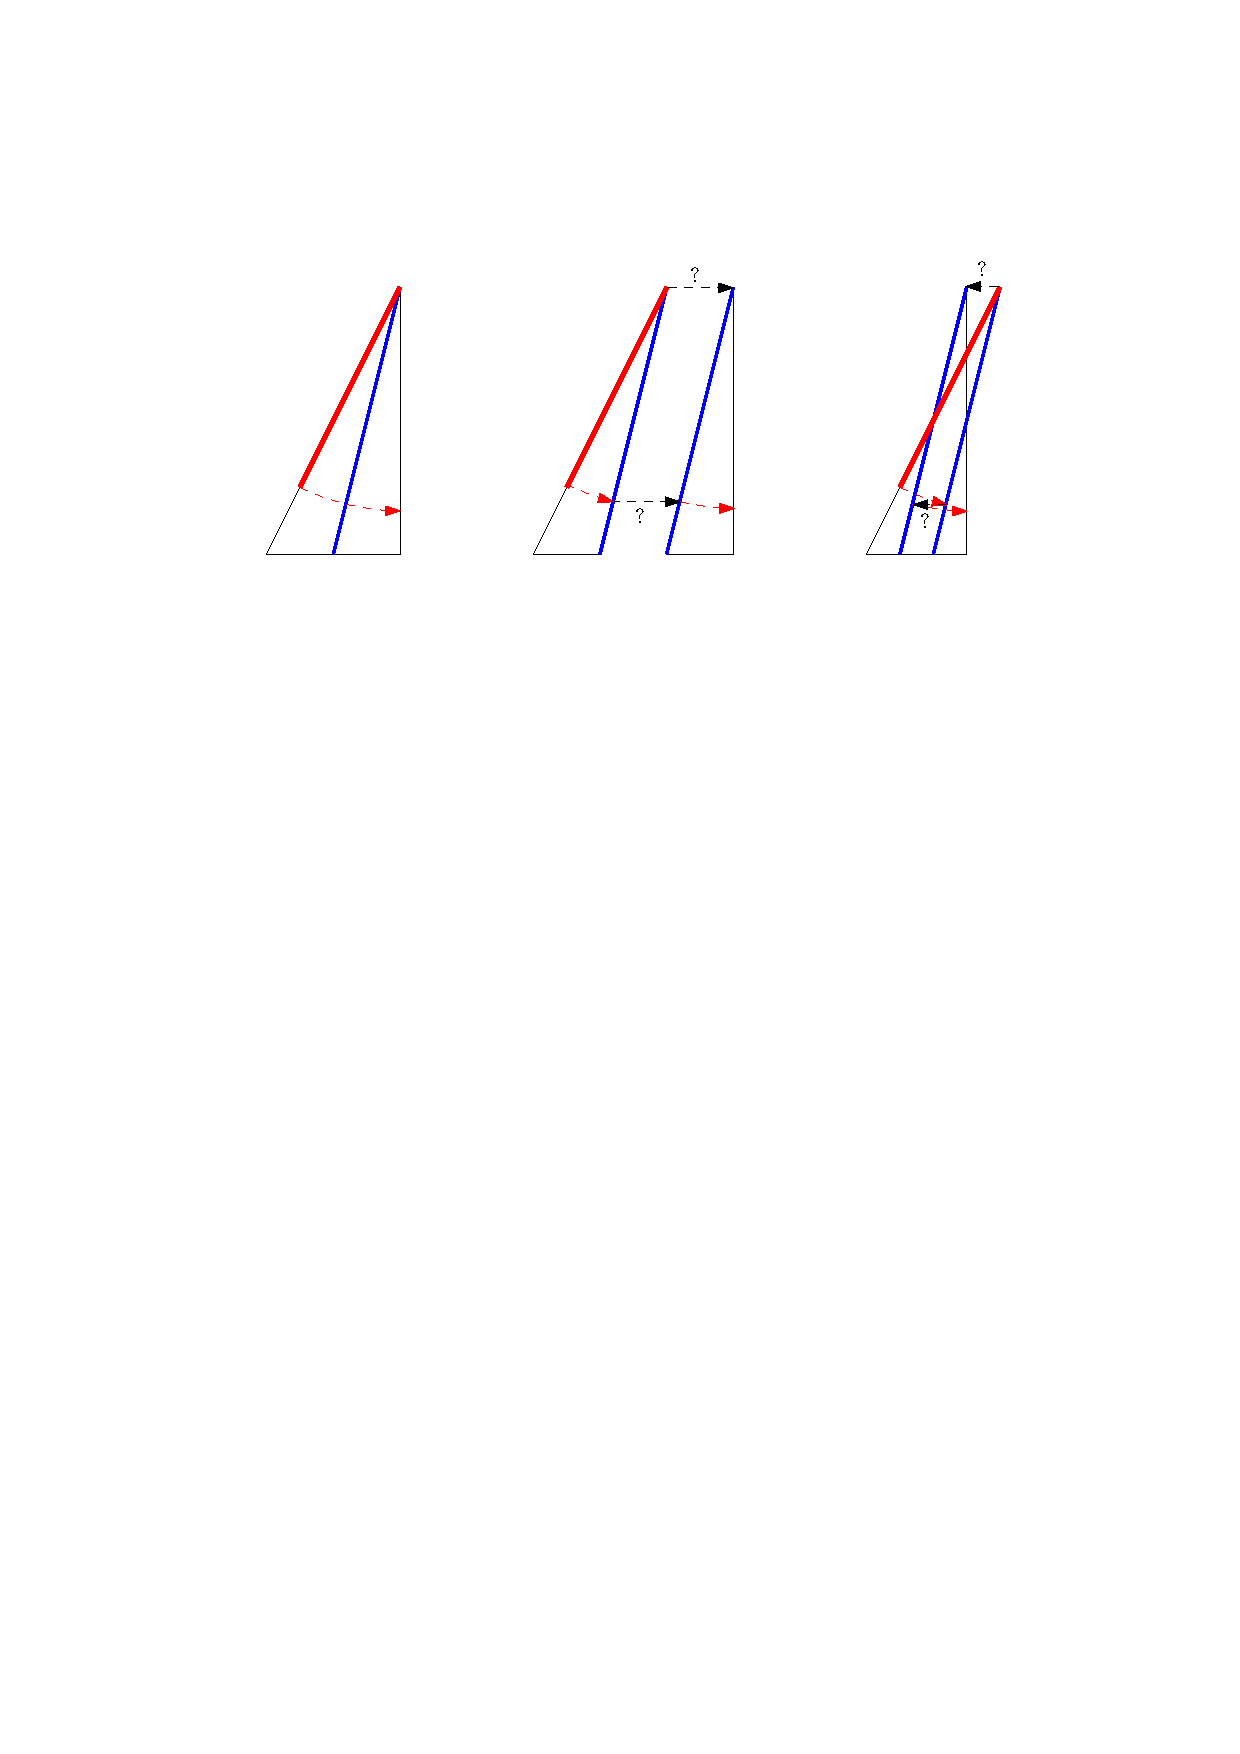
\includegraphics[width=0.7\textwidth]{ipe_slike/preskok1.pdf}
    \caption{Možne translacije sosednjih podtrikotnikov in vrtenje daljice skozi njiju}
    \label{preskok1}
\end{figure}

%%%%%%%%%%%%%%%%%%%%%%%%%%%%%%%%%%%%%%%%%%%%%%%%%%%%%%%%%%%%%%%%%

\section*{Preskok daljice med sosednjima trikotnikoma}

Pál je za preskakovanje daljice med dvema sosednjima podtrikotnikoma, ki se ne stikata več na skupni stranici (sredinski in desni primer na sliki~\ref{preskok1}), podal nadvse enostavno rešitev v naslednjih dveh korakih (gl. sliko~\ref{pal}):

\begin{enumerate}
    \item \textbf{Konstrukcija Pálovega spoja} (zeleno območje): Nad prekrivajočima sosednjima podtrikotnikoma narišemo nosilki obeh modrih stranic, ki sta seveda vzporedni. Nato zarišemo daljico, ki ju povezuje, kot je narisano na sliki.
    \item \textbf{Gibanje po črki ``N''}: Ko se enotska daljica obrne v vrhu prvega podtrikotnika in pristane na modri stranici, jo pošljemo po prvi nosilki do začetka povezovalne daljice, kjer jo zavrtimo okoli zgornjega krajišča, da pristane na povezovalni daljici, nato jo premaknemo po tej daljici do vrha drugega podtrikotnika, jo zavrtimo v nasprotno smer, da pristane na drugi nosilki, po kateri jo nato potisnemo v drugi podtrikotnik.
\end{enumerate}

\begin{figure}[h!]
    \centering
    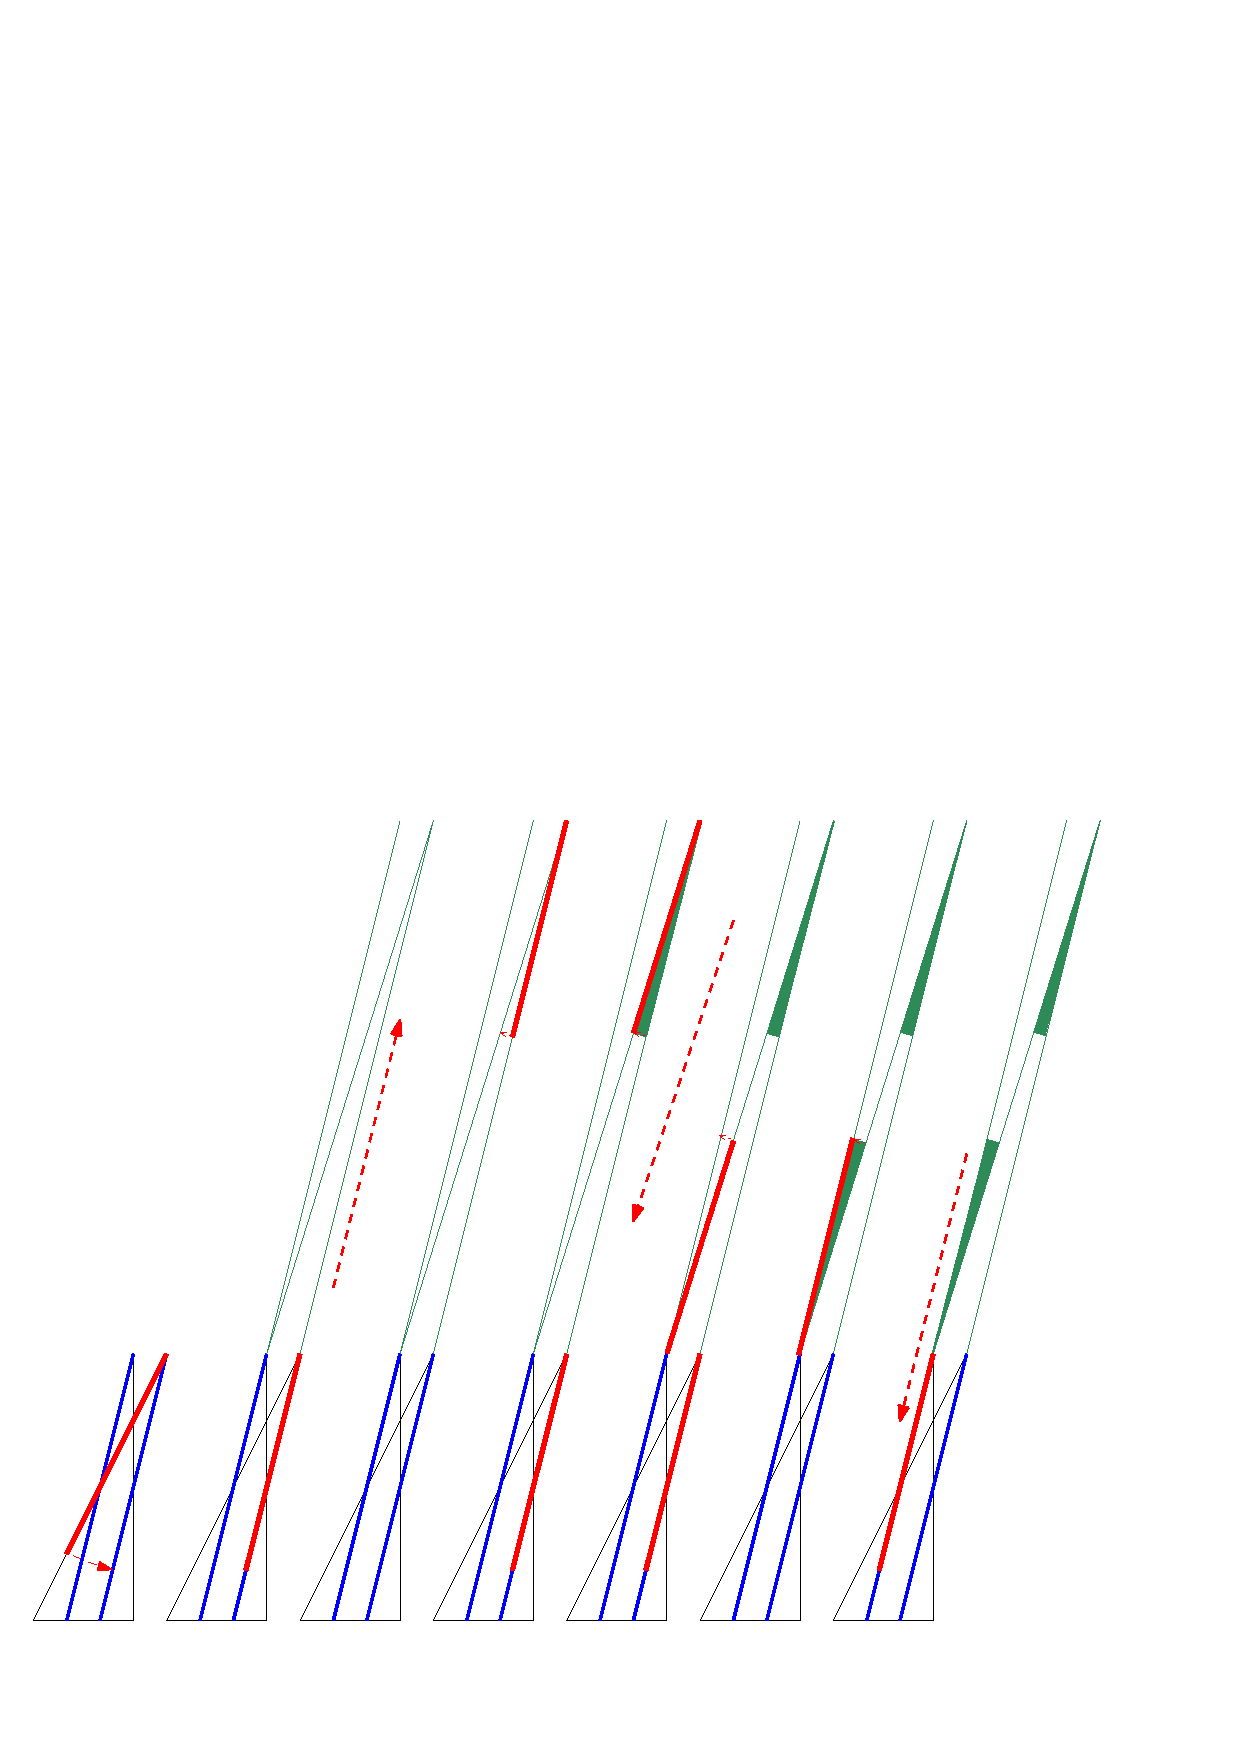
\includegraphics[width=\textwidth]{ipe_slike/pal.pdf}
    \caption{Preskok daljice preko Pálovega spoja}
    \label{pal}
\end{figure}

Smer enotske daljice se na ta način pri preskoku v sosednji podtrikotnik ohrani, daljica pa med tem prehodom (gibanjem po zelenem liku) opiše poljubno majhno ploščino, saj je kot vrtenja, če za zgornje krajišče povezovalne daljice izberemo poljubno oddaljeno točko na prvi nosilki, lahko poljubno majhen ter s tem tudi ploščina orisanega krožnega izseka, daljice pa k skupni ploščini tako ali tako ne prispevajo ničesar.

\textbf{Torej za vsak preskok enotske daljice med sosednjima podtrikotnikoma \emph{potrebujemo} (in znamo konstruirati) \emph{dodatno ploščino}, vendar je le-ta lahko \emph{poljubno majhna}.}

%%%%%%%%%%%%%%%%%%%%%%%%%%%%%%%%%%%%%%%%%%%%%%%%%%%%%%%%%%%%%%%%%

\section*{Perronovo drevo}

S Pálovimi spoji smo rešili težavo vzporednih translacij enotske daljice, pri čemer se je skupna ploščina lika povečala le za poljubno majhno vrednost. Zanima nas še, kako medsebojno prekriti podtrikotnike, da bo tudi ploščina celotnega območja prekritja poljubno majhna; s tem bo vprašanje Kakeye odgovorjeno. Tu nam pride v pomoč preprosta, a zanimiva konstrukcija, ki si jo je zamislil Perron, zato je po njem poimenovana \textbf{Perronovo drevo}.

\begin{wrapfigure}{r}{0.23\textwidth}
    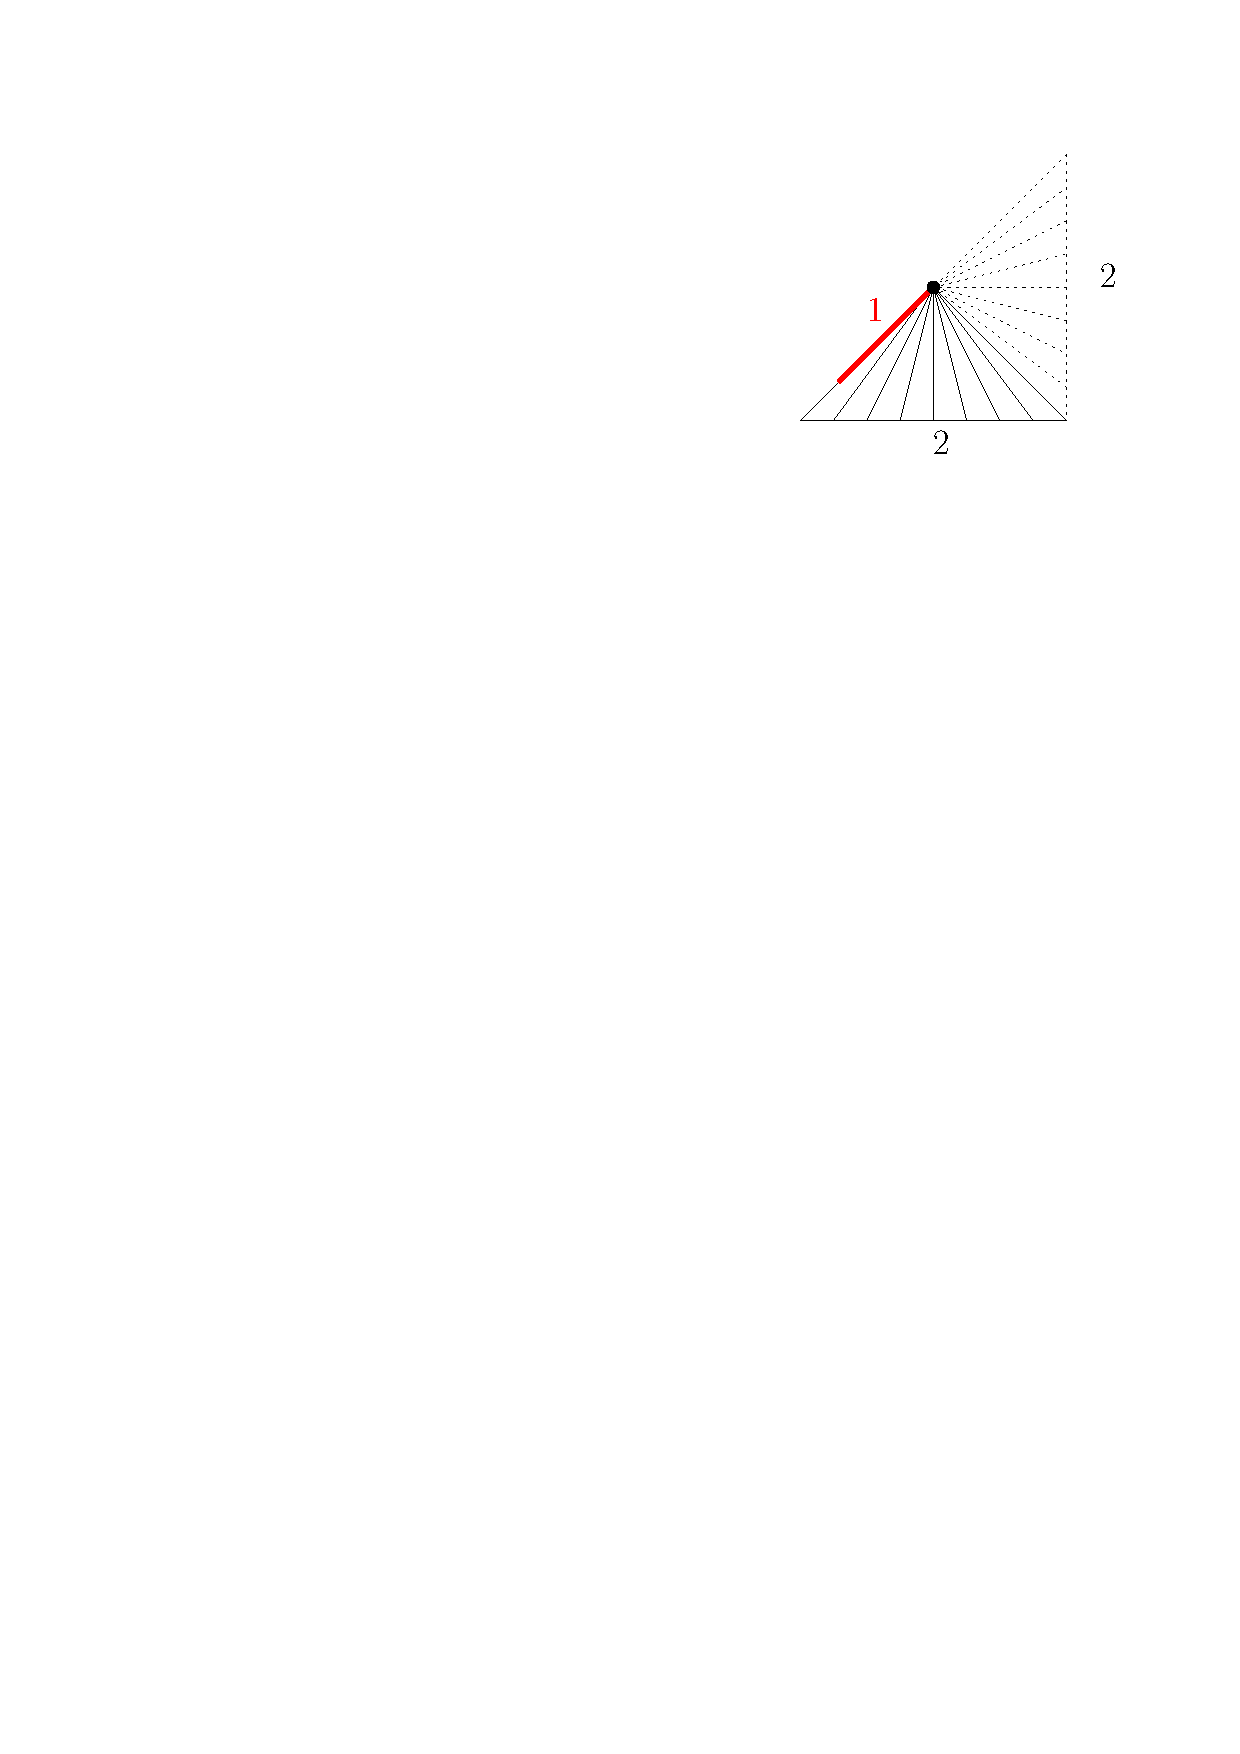
\includegraphics[width=0.9\linewidth]{ipe_slike/polovica_trikotnika.pdf}
\end{wrapfigure}

Spomnimo se, kako smo iz pravokotnega enakokrakega trikotnika dobili $ 2n $ manjših trikotnikov (slika~\ref{trikotnik_razdelitev}). Vzemimo spodnji osnovni trikotnik, ki je na desni označen z neprekinjeno črto, in na njem poglejmo konstrukcijo. Za drugi osnovni trikotnik, ki je pravokoten na prvega, bo postopek enak.

\begin{wrapfigure}{l}{0.45\textwidth}
    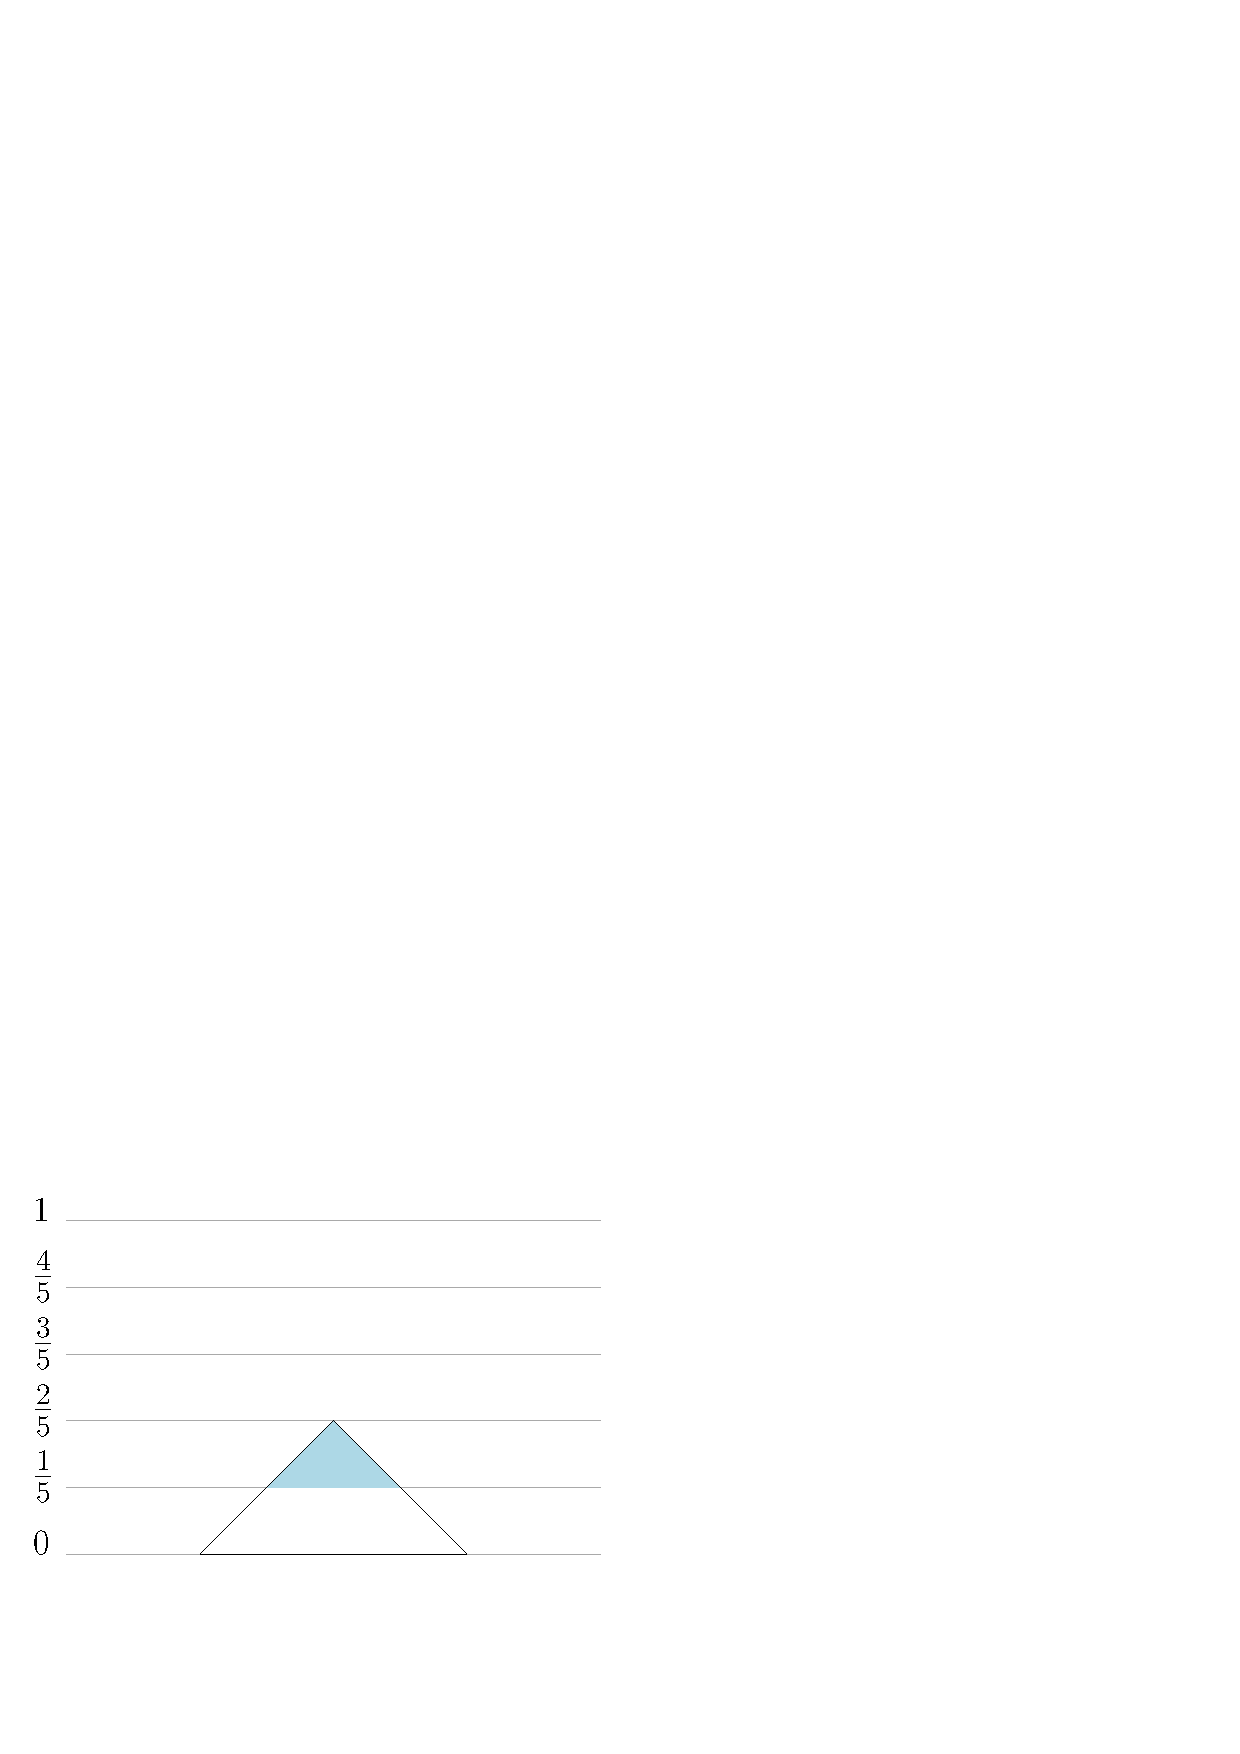
\includegraphics[width=0.9\linewidth]{ipe_slike/k_5.pdf}
    \caption{Koordinatni sistem ($ k = 5 $)}
    \label{sistem5}
\end{wrapfigure}

Pri konstrukciji bomo povečevali število podtrikotnikov, na katere je razdeljen osnovni trikotnik. Naj bo $ k \in \mathbb{N}, k \geq 2 $, in naš koordinatni sistem tak, kot ga kaže slika~\ref{sistem5}: v vertikalni smeri je razdalja 1 razdeljena na $ k $ skladnih delov -- ``nivojev''. Na spodnjo horizontalno črto položimo osnovnemu trikotniku podoben trikotnik z višino $ \frac{2}{k} $.

Definirajmo še \emph{vrh} -- to je vsak trikotnik z višino $ \frac{1}{k} $, ki v koordinatnem sistemu leži najvišje (na sliki ~\ref{sistem5} pobarvan modro).

Z naslednjim postopkom zgeneriramo osnovni trikotnik z višino 1, ki je razdeljen na medsebojno že premaknjenih $ n = 2^{k-2} $ podtrikotnikov: \emph{Nehorizontalni stranici vsakega vrha podaljšamo za en nivo navzgor in dobljeni zgornji krajišči povežemo s spodnjima ogliščema vrha, kot kaže slika~\ref{koraki} (torej se spustimo za dva nivoja navzdol). Tako vrh dobi dva ``uhlja''.}

Postopek ponovimo za vsak nov vrh, dokler ne pridemo do nivoja 1, torej ko opravimo $ k-2 $ korakov. Celoten proces imenujemo \textbf{brstenje Perronovega drevesa}.

\begin{figure}[h!]
    \centering
    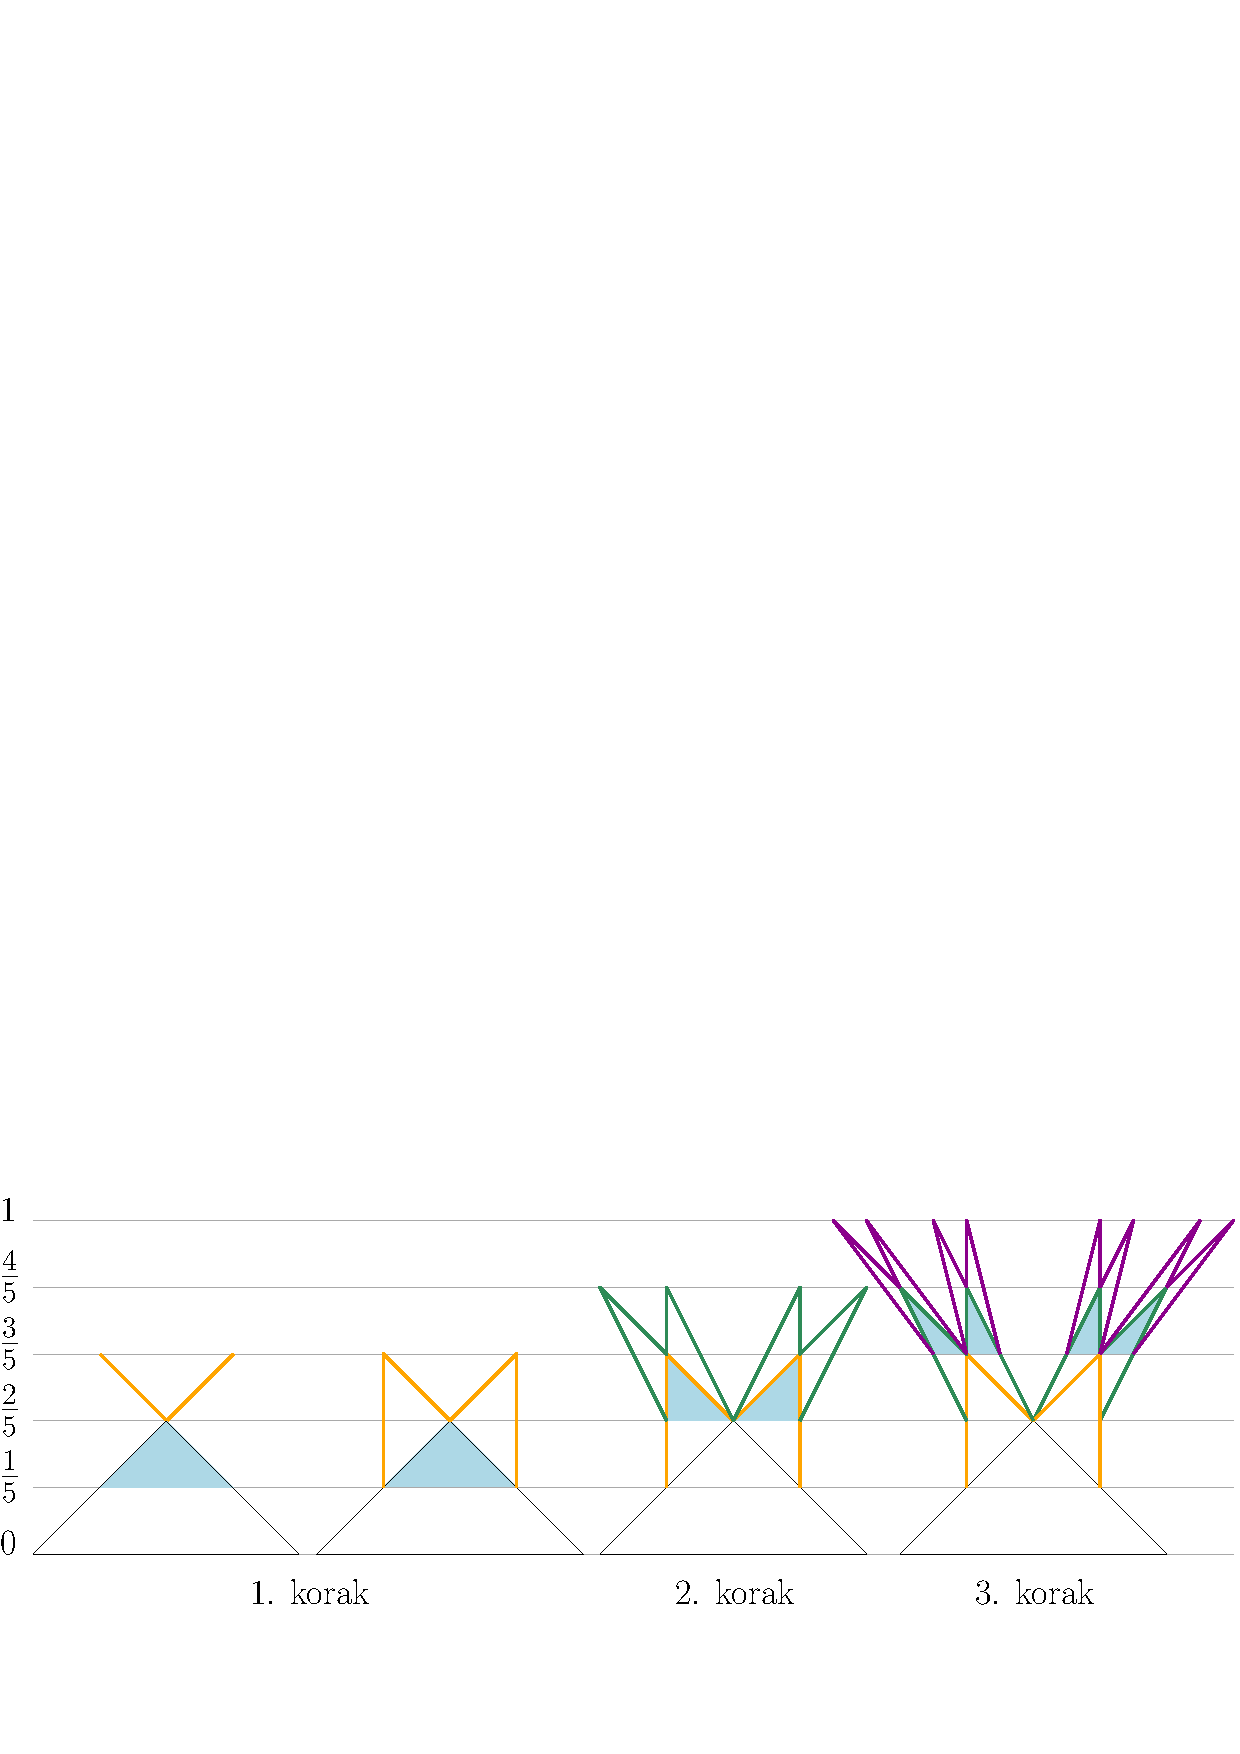
\includegraphics[width=0.9\textwidth]{ipe_slike/koraki.pdf}
    \caption{Generiranje osnovnega trikotnika in podtrikotnikov za $ k = 5 $}
    \label{koraki}
\end{figure}

\noindent Sedaj moramo premisliti naslednje lastnosti te konstrukcije:

\begin{enumerate}
    \item Vsak vrh porodi skadna uhlja, ki imata enako ploščino kot taisti vrh.
    \item V $ l $-tem koraku ($ l = 1, 2, \ldots, k-2 $) dobimo $ 2^l $ prekrivajočih se podtrikotnikov, ki skupaj sestavijo osnovnemu trikotniku podoben trikotnik z višino $ \frac{l+2}{k} $.
    \item V vsakem koraku se nam skupna ploščina poveča za natanko dvakratno ploščino vrha, s katerim začnemo prvi korak (slika~\ref{koraki}), tj. za $ \frac{2}{k^2} $.
    \item Skupna ploščina lika, ki ga dobimo na zadnjem koraku, je $ \frac{2}{k} $.
\end{enumerate}

%%%%%%%%%%%%%%%%%%%%%%%%%%%%%%%%%%%%%%%%%%%%%%%%%%%%%%%%%%%%%%%%%

\subsubsection*{Lastnost 1}

Poglejmo si uhlja, ki nastaneta na nekem vmesnem koraku iz enega od vrhov ((a) na sliki~\ref{uhlji}):

\begin{itemize}
    \item \emph{Ploščina uhljev} (b): Vsak trikotnik, sestavljen iz vrha in enega izmed uhljev (označeno z zeleno), ima dvakratno ploščino vrha, saj je osnovnica skupna, višina pa dvakrat večja od višine vrha. Torej ima vsak uhelj enako ploščino kot vrh.
    \item \emph{Skladnost uhljev} (c): Zaradi podaljšanja stranic uhljev za en nivo navzgor imata uhlja dva para skladnih stranic ob sovršnem kotu, torej sta res skladna in sta njuni najdaljši stanici vzporedni.
\end{itemize}

\begin{figure}[h!]
    \centering
    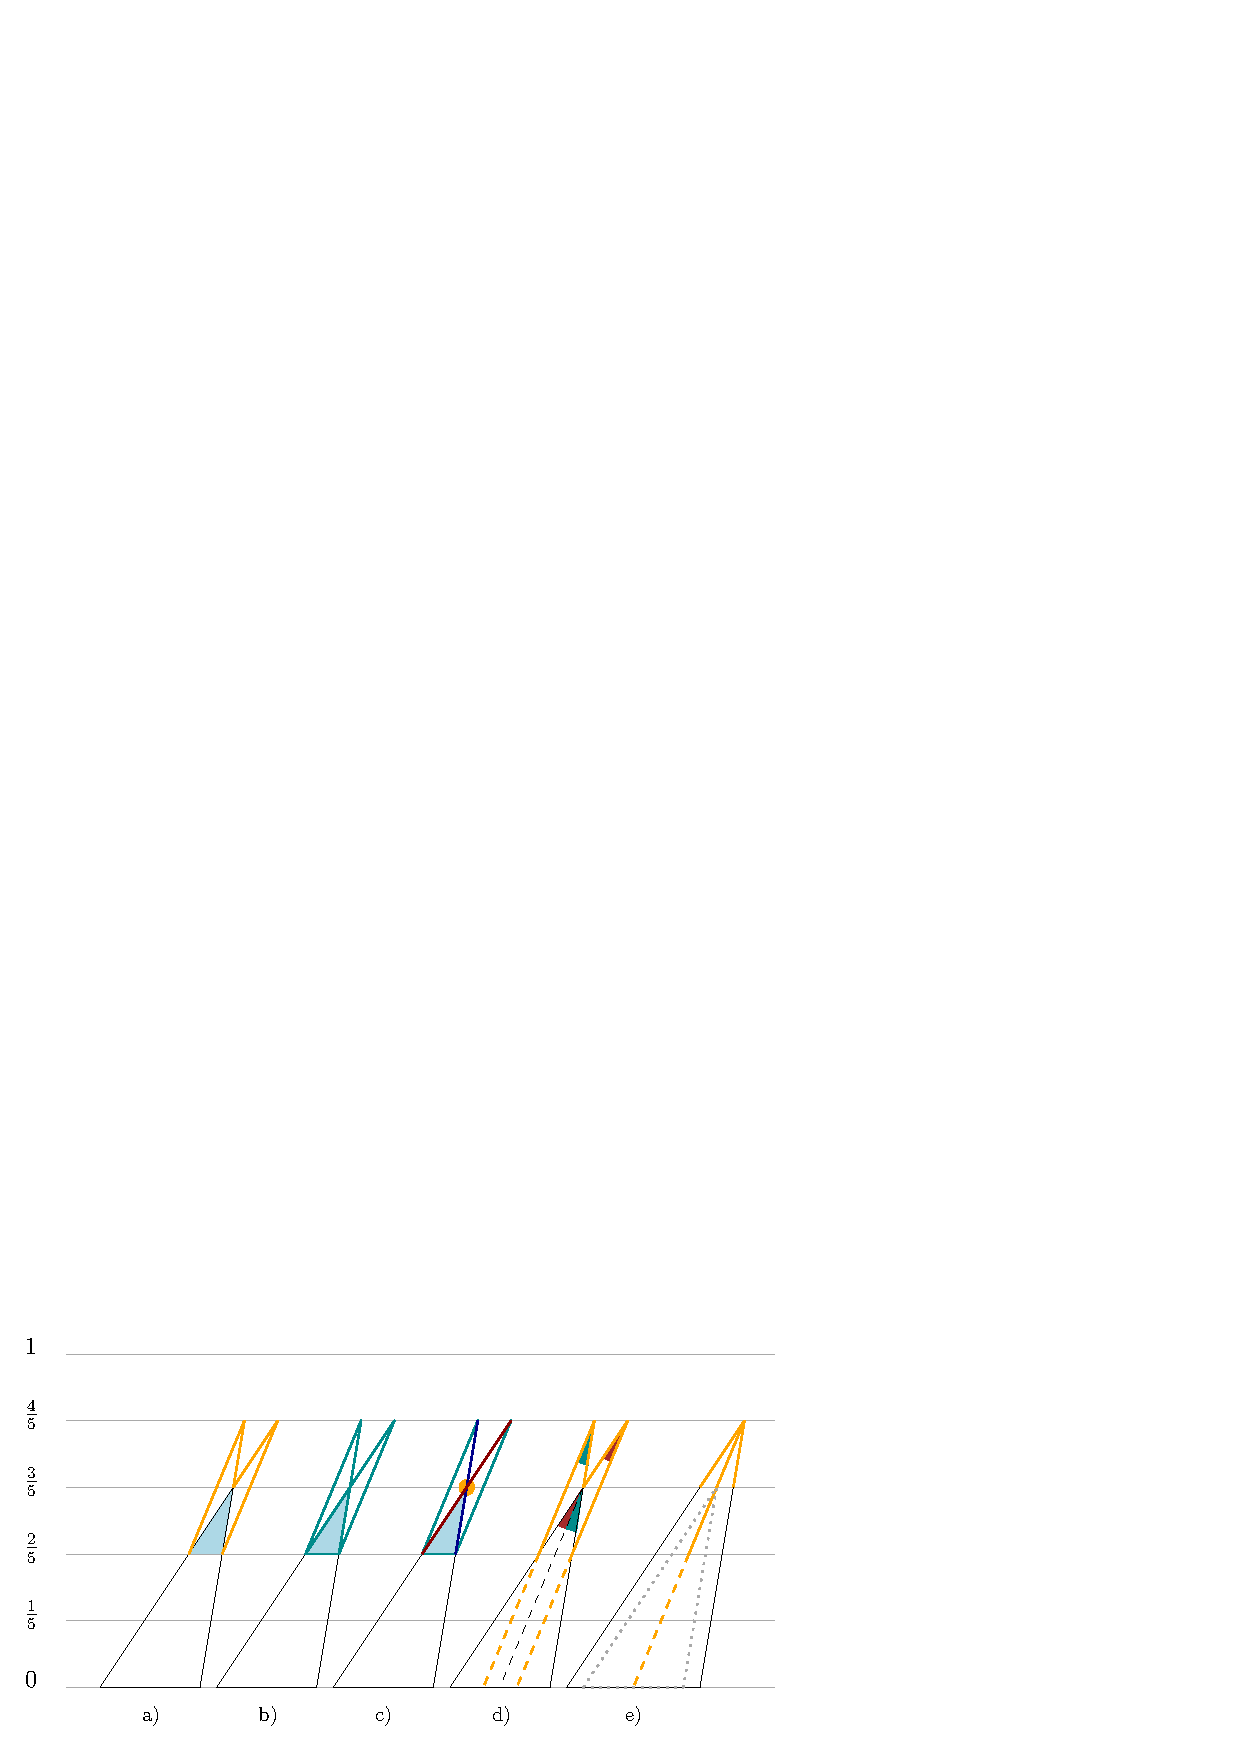
\includegraphics[width=0.75\textwidth]{ipe_slike/uhlji.pdf}
    \caption{Geometrijski dokaz lastnosti 1}
    \label{uhlji}
\end{figure}

Iz skladnosti sledi, sta tudi oranžni črtkani nosilki (d) vzporedni in smo res dobili dva sosednja podtrikotnika, ki skupaj tvorita trikotnik, podoben prejšnjemu (e), le za $ \frac{1}{k} $ višji.

%%%%%%%%%%%%%%%%%%%%%%%%%%%%%%%%%%%%%%%%%%%%%%%%%%%%%%%%%%%%%%%%%

\subsubsection*{Lastnost 2}

Ker postopek začnemo s trikotnikom, ki je podoben osnovnemu trikotniku, in ker iz lastnosti 1 sledi, da na vsakem koraku iz enega trikotnika dobimo dva višja podtrikotnika, ki skupaj tvorita njemu podoben trikotnik, v $ l $-tem koraku res dobimo $ 2^l $ podtrikotnikov, ki skupaj sestavijo ustrezno pomanjšan osnovni trikotnik (slika~\ref{lastnost2}). Njihova višina je $ \frac{l+2}{k} $, saj prvi korak začnemo na višini $ \frac{2}{k} $ in se vsakič dvignemo za $ \frac{1}{k} $ navzgor. V zadnjem koraku tako res dobimo $ 2^{k-2} $ podtrikotnikov.

\begin{figure}[h!]
    \centering
    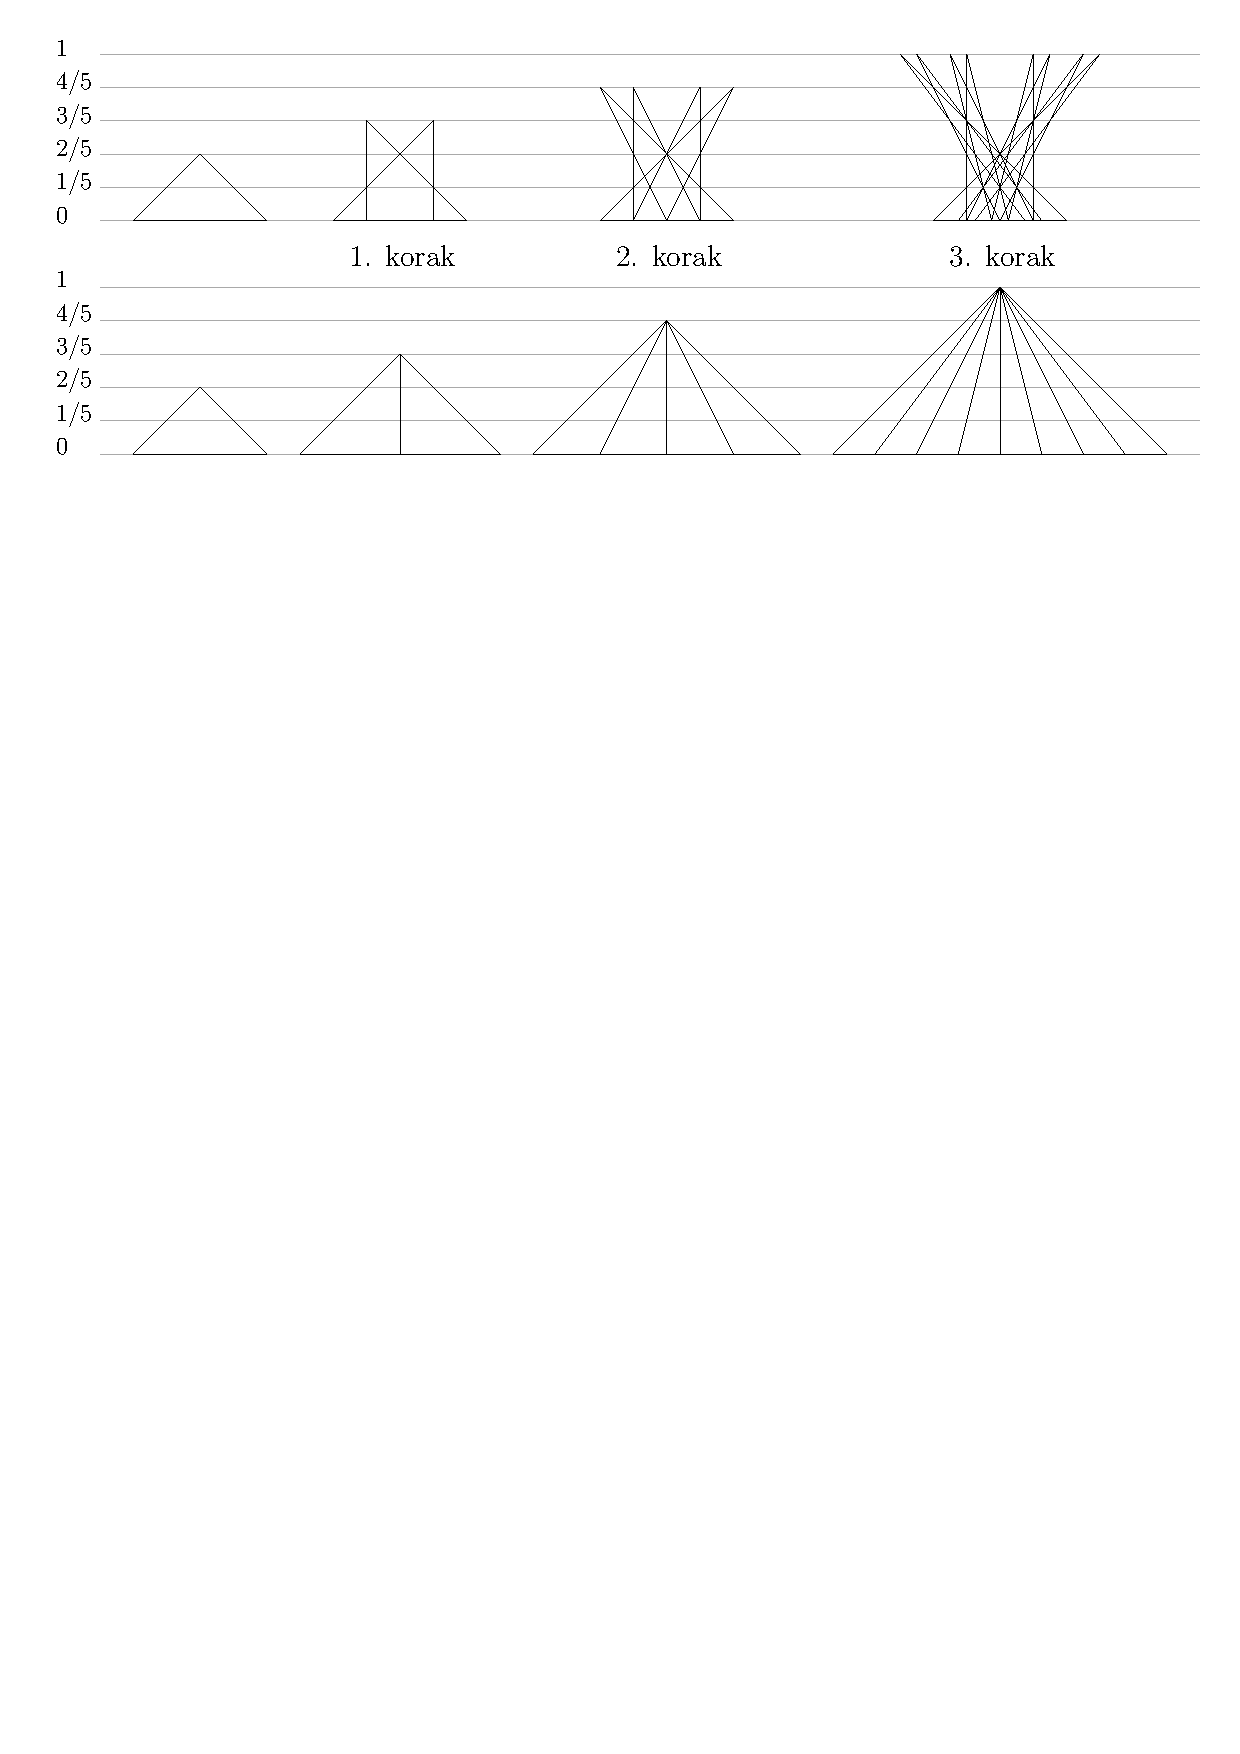
\includegraphics[width=\textwidth]{ipe_slike/lastnost2.pdf}
    \caption{Geometrijski prikaz lastnosti 2 za $ k = 5 $}
    \label{lastnost2}
\end{figure}

%%%%%%%%%%%%%%%%%%%%%%%%%%%%%%%%%%%%%%%%%%%%%%%%%%%%%%%%%%%%%%%%%

\subsubsection*{Lastnost 3}

Iz konstrukcije in podobnosti je razvidno, da vsak vrh preko uhljev porodi dva vrhova, ki sta (če ju zlepimo skupaj) skladna taistemu vrhu (slika~\ref{vrhovi}). Zato na vsakem koraku vsi novi vrhovi skupaj tvorijo ravno originalen vrh, s katerim smo začeli. Ker ima vsak nov vrh polovično ploščino uhlja, se na vsakem koraku ploščina poveča za dvakratno skupno ploščino novih vrhov, torej za dvakratno ploščino originalnega vrha, tj. za $ 2 \left( \frac{1}{2} \cdot \frac{2}{k} \cdot \frac{1}{k} \right) = \frac{2}{k^2} $.

\begin{figure}[h!]
    \centering
    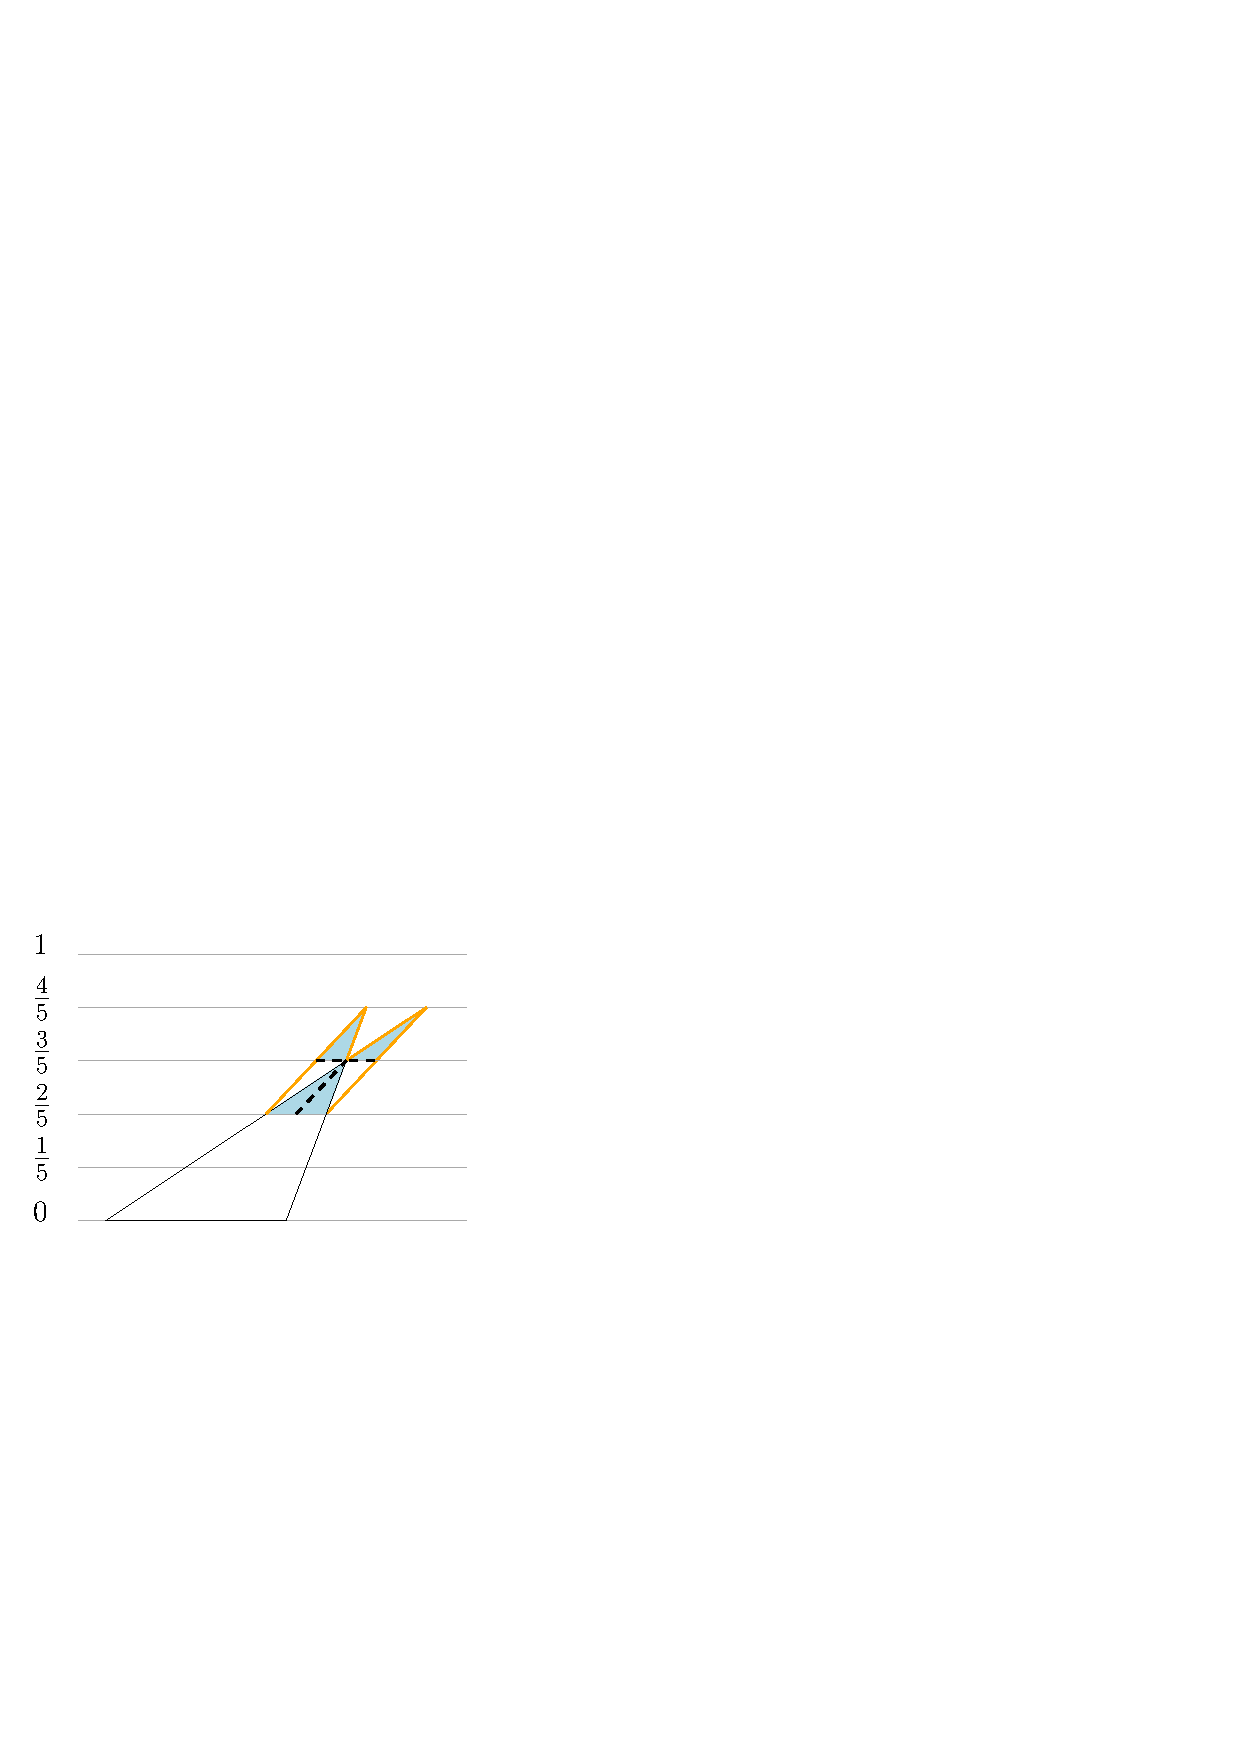
\includegraphics[width=0.4\textwidth]{ipe_slike/novi_vrhovi.pdf}
    \caption{Vsak vrh porodi vrhova, ki sta mu (zlepljena skupaj) skladna}
    \label{vrhovi}
\end{figure}

%%%%%%%%%%%%%%%%%%%%%%%%%%%%%%%%%%%%%%%%%%%%%%%%%%%%%%%%%%%%%%%%%

\subsubsection*{Lastnost 4}

Skupna ploščina je tako sestavljena iz ploščine prvotnega trikotnika z višino $ \frac{2}{k} $ in iz na vsakem koraku dodanih enakih ploščin. Opravili smo $ (k-2) $ korakov, torej je skupna ploščina Perronovega drevesa za izbrani $ k $ enaka

\begin{equation*}
    S = \frac{1}{2} \cdot \frac{4}{k} \cdot \frac{2}{k}  + (k -2) \cdot \frac{2}{k^2} = \frac{2}{k}.
\end{equation*}

S to konstrukcijo smo prišli do odgovora na Kakeyino vprašanje, ki ga je podal že Besicovitch. Večji kot je $ k $, manjša je skupna ploščina lika in posledično lahko dobimo poljubno majhno ploščino. Na sliki~\ref{brstenje_n_k} lahko opazujemo, kako se Perronovo drevo s povečevanjem $ k $ oz. števila razdelitev osnovnega trikotnika na podtrikotnike vse bolj razvejuje, ploščina pa manjša.

\begin{figure}[h!]
    \centering
    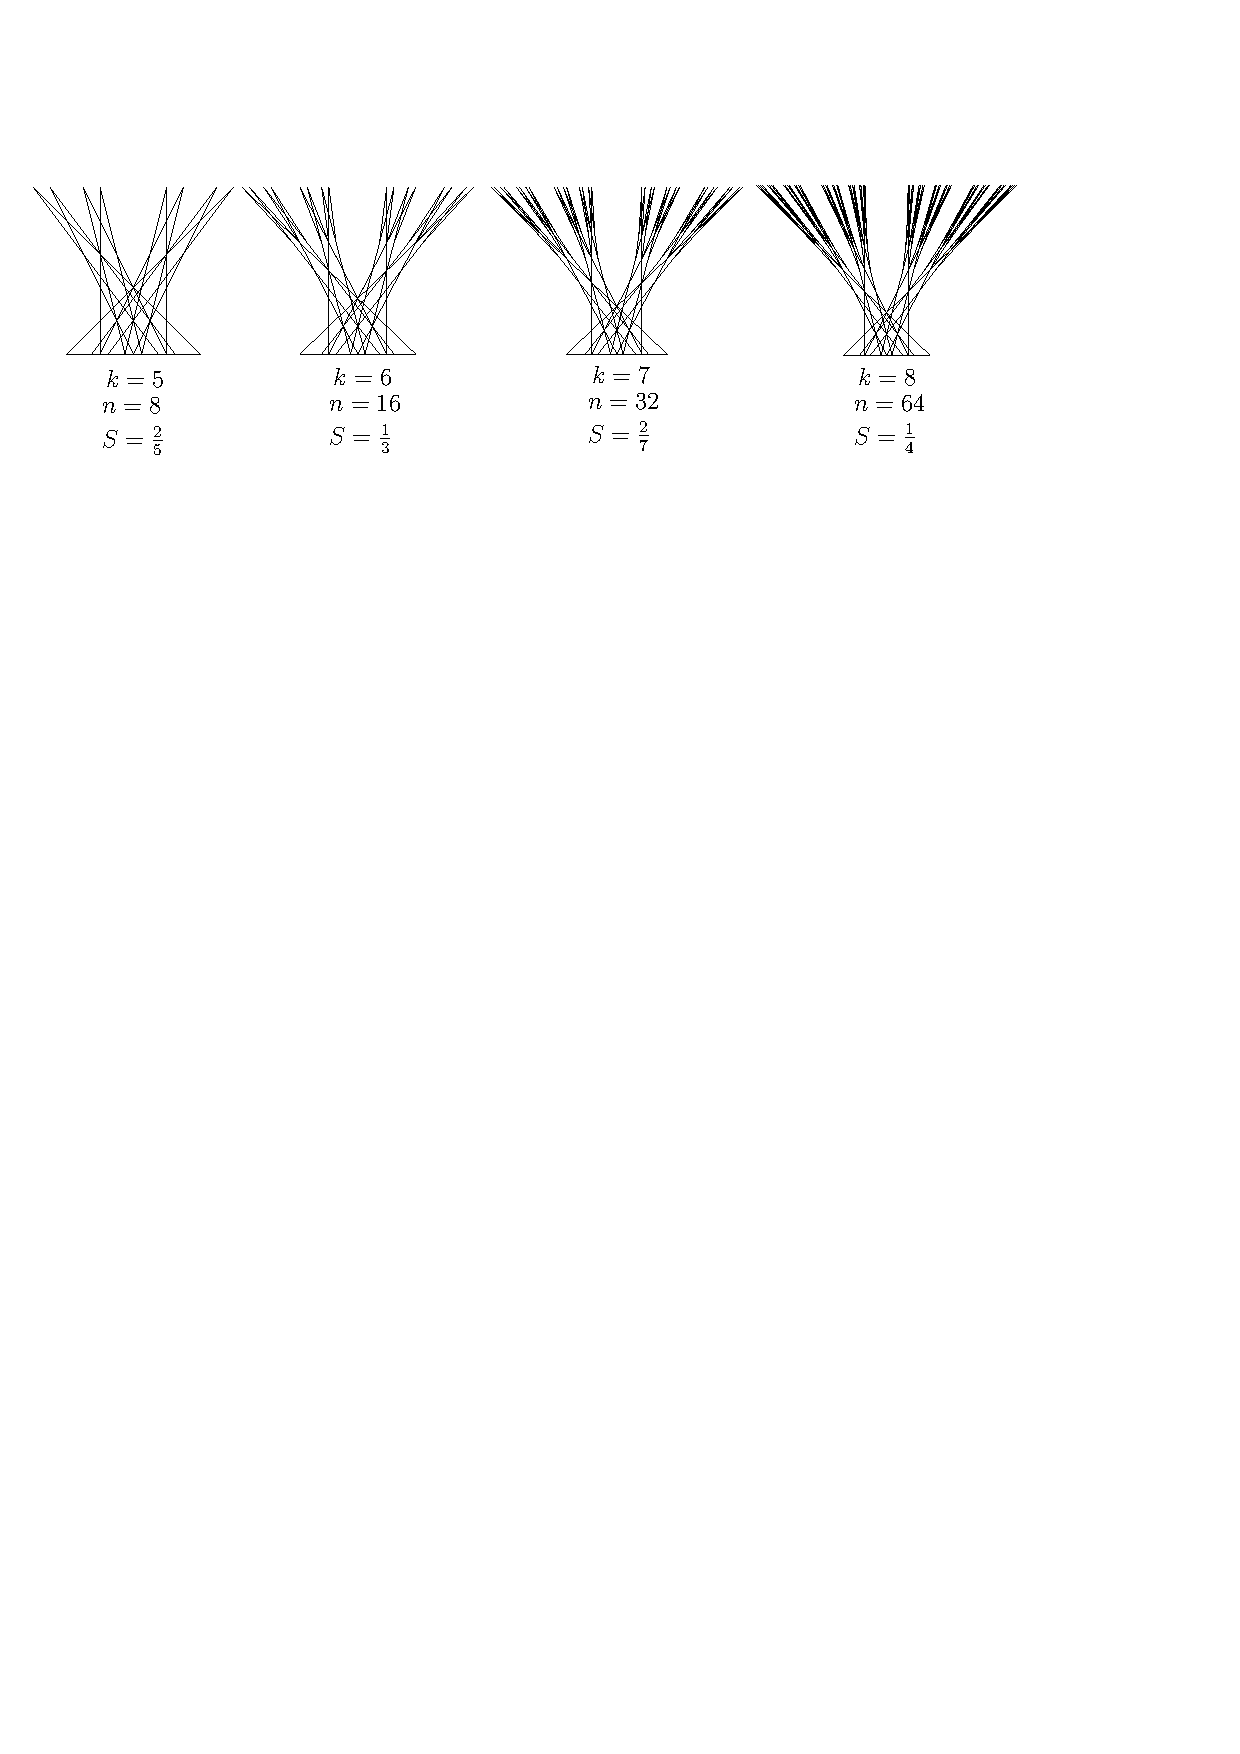
\includegraphics[width=\textwidth]{ipe_slike/brstenje_k_n.pdf}
    \caption{Perronova drevesa za $ k = 5, 6, 7, 8 $}
    \label{brstenje_n_k}
\end{figure}

%%%%%%%%%%%%%%%%%%%%%%%%%%%%%%%%%%%%%%%%%%%%%%%%%%%%%%%%%%%%%%%%%
\newpage

\section*{Povzetek rezultatov in slika konstrukcije}

Za konstrukcijo lika, v katerem se enotska daljica zvezno obrne za 180°, uporabimo Perronovo drevo. Izberemo $ k \in \mathbb{N}, k \geq 2, $ in preko brstenja drevesa tvorimo $ n = 2^{k-2} $ podtrikotnikov z višino 1, na katere je razdeljen osnovni trikotnik z višino 1 (slika~\ref{brstenje}). Ploščina dobljenega lika je $ \frac{2}{k} $.

\begin{figure}[h!]
    \centering
    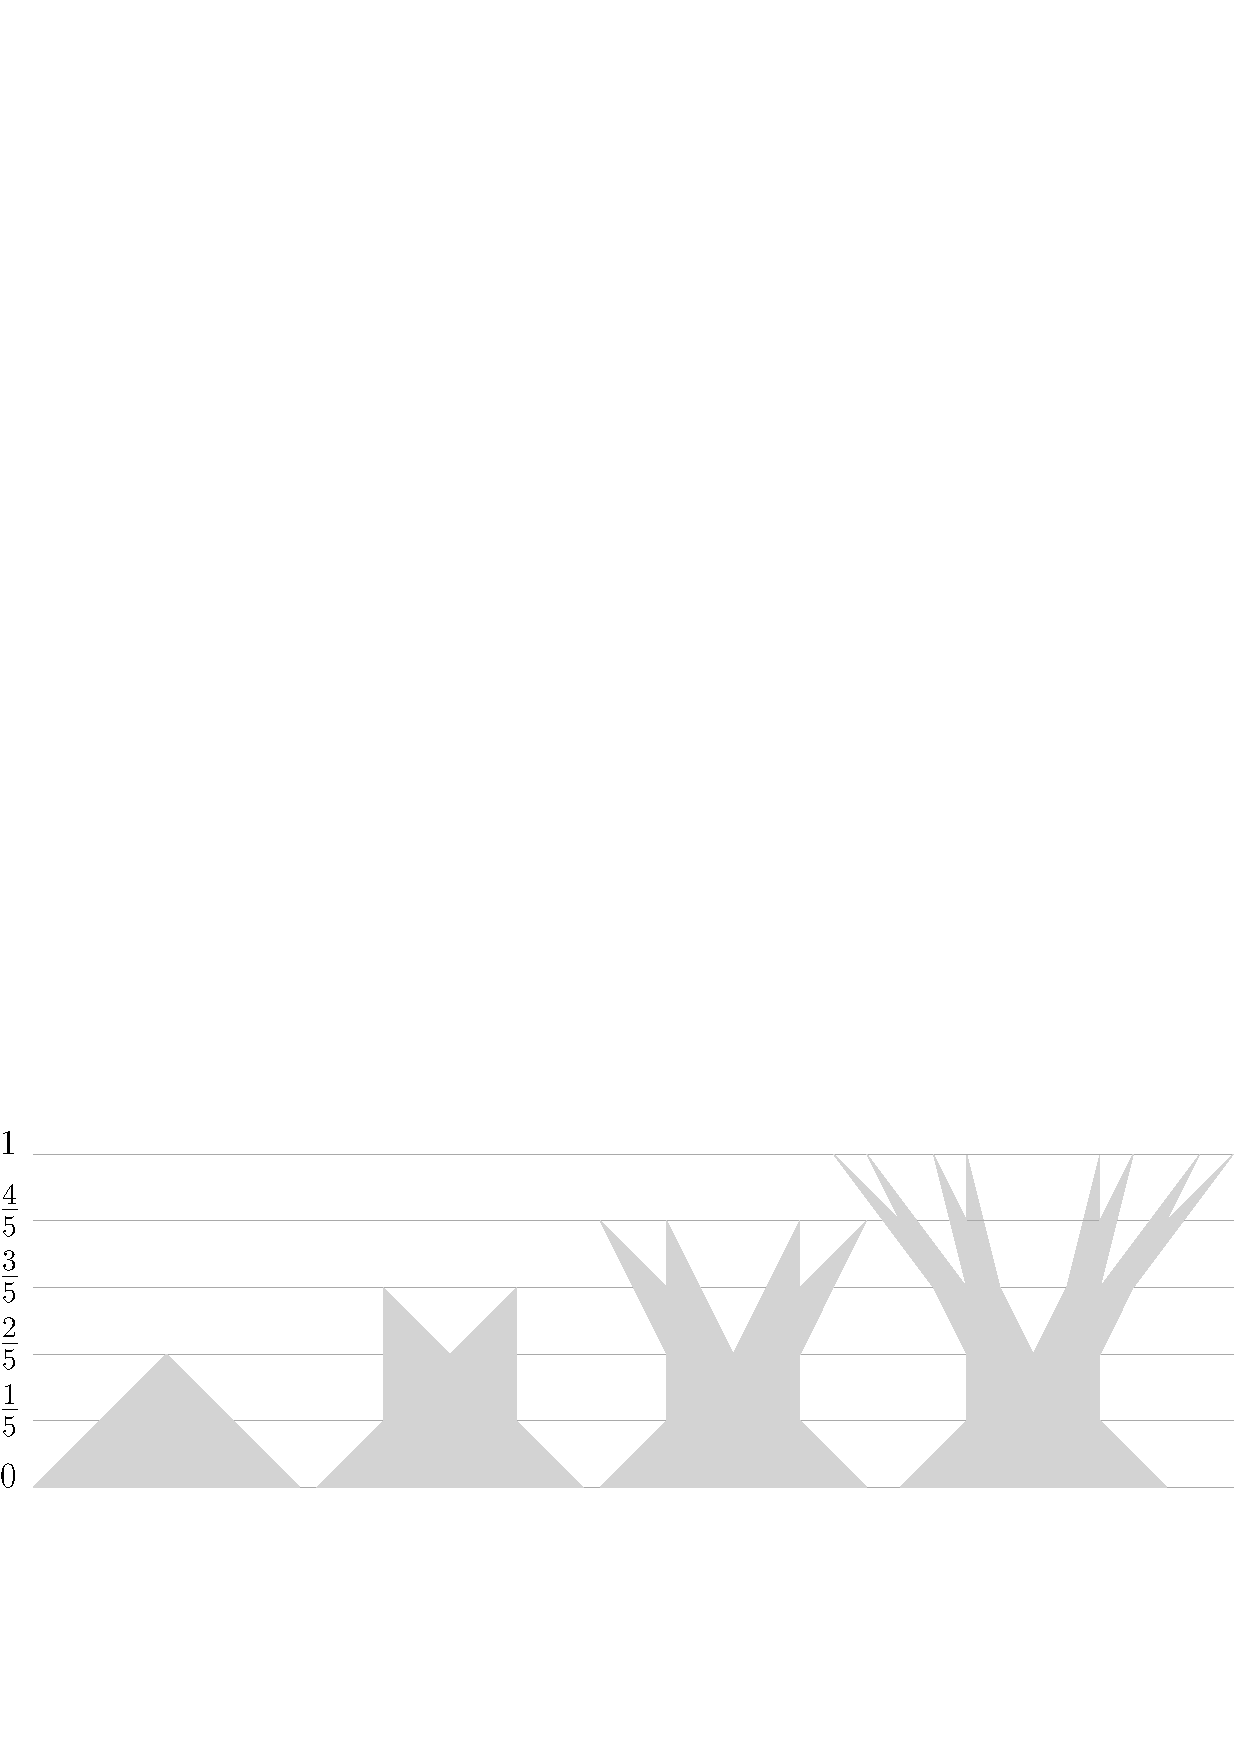
\includegraphics[width=0.8\textwidth]{ipe_slike/perronova_drevesa.pdf}
    \caption{Brstenje Perronovega drevesa za $ k = 5 $}
    \label{brstenje}
\end{figure}

Za prehod enotske daljice med sosednjimi podtrikotniki potrebujemo še $ n-1 $ Pálovih spojev, ki pa skupaj doprinesejo poljubno majhno ploščino. Na sliki~\ref{prehodi} je prikazano, kako se enotska daljica zvezno zavrti za 90° znotraj enega osnovnega trikotnika (z rdečo je označen njen začetni, z modro pa končni položaj). S prekinjeno črto so označeni Pálovi spoji, ki jih je res sedem. Premikanje torej poteka za vsak podtrikotnik enako -- najprej se daljica zasuče okoli zgornjega oglišča, da pade na drugo stranico, nato pa preko spoja preide v naslednji podtrikotnik.

\begin{figure}[h!]
    \centering
    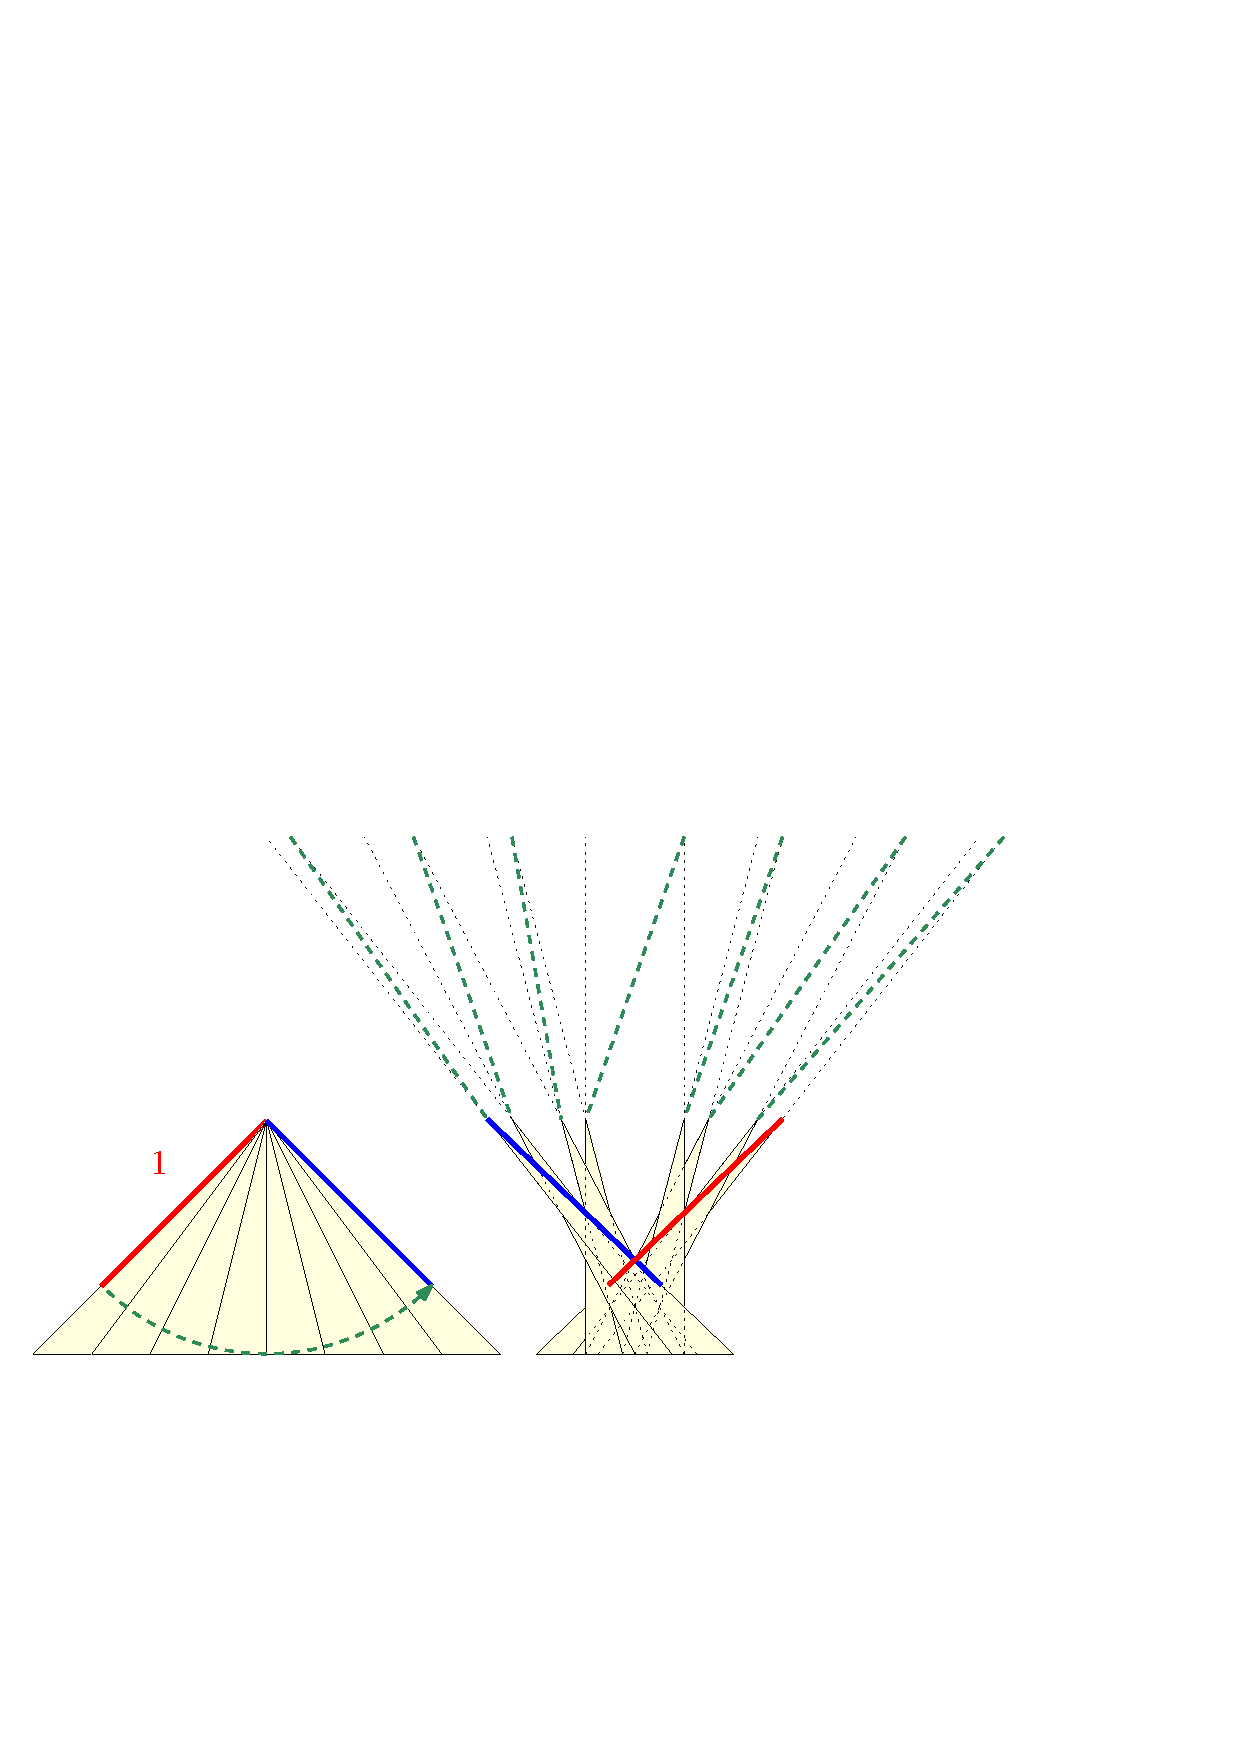
\includegraphics[width=0.9\textwidth]{ipe_slike/prehod_drevo1.pdf}
    \caption{Rotacija enotske daljice za 90° pri $ n = 8 $}
    \label{prehodi}
\end{figure}

Postopek ponovimo še na drugem osnovnem trikotniku, ki je pravokoten na prvega. Lika preko Pálovega spoja združimo, na primer kot kaže slika~\ref{zdruzitev}. Ko se daljica zavrti za 180°, jo samo potisnemo po isti stranici na začetno pozicijo in postopek ponovimo, da dobimo obrat enotske daljice za 360°. Končni lik ima ploščino največ $ \frac{4}{k} + \epsilon $, kjer je $ \epsilon $ skupna, a poljubno majhna ploščina, ki jo prispeva $ 2n - 1 $ Pálovih spojev. Ko povečujemo $ k $, gre skupna ploščina proti nič (vendar nikoli ne dosežemo ničelne ploščine!).

\begin{figure}[h!]
    \centering
    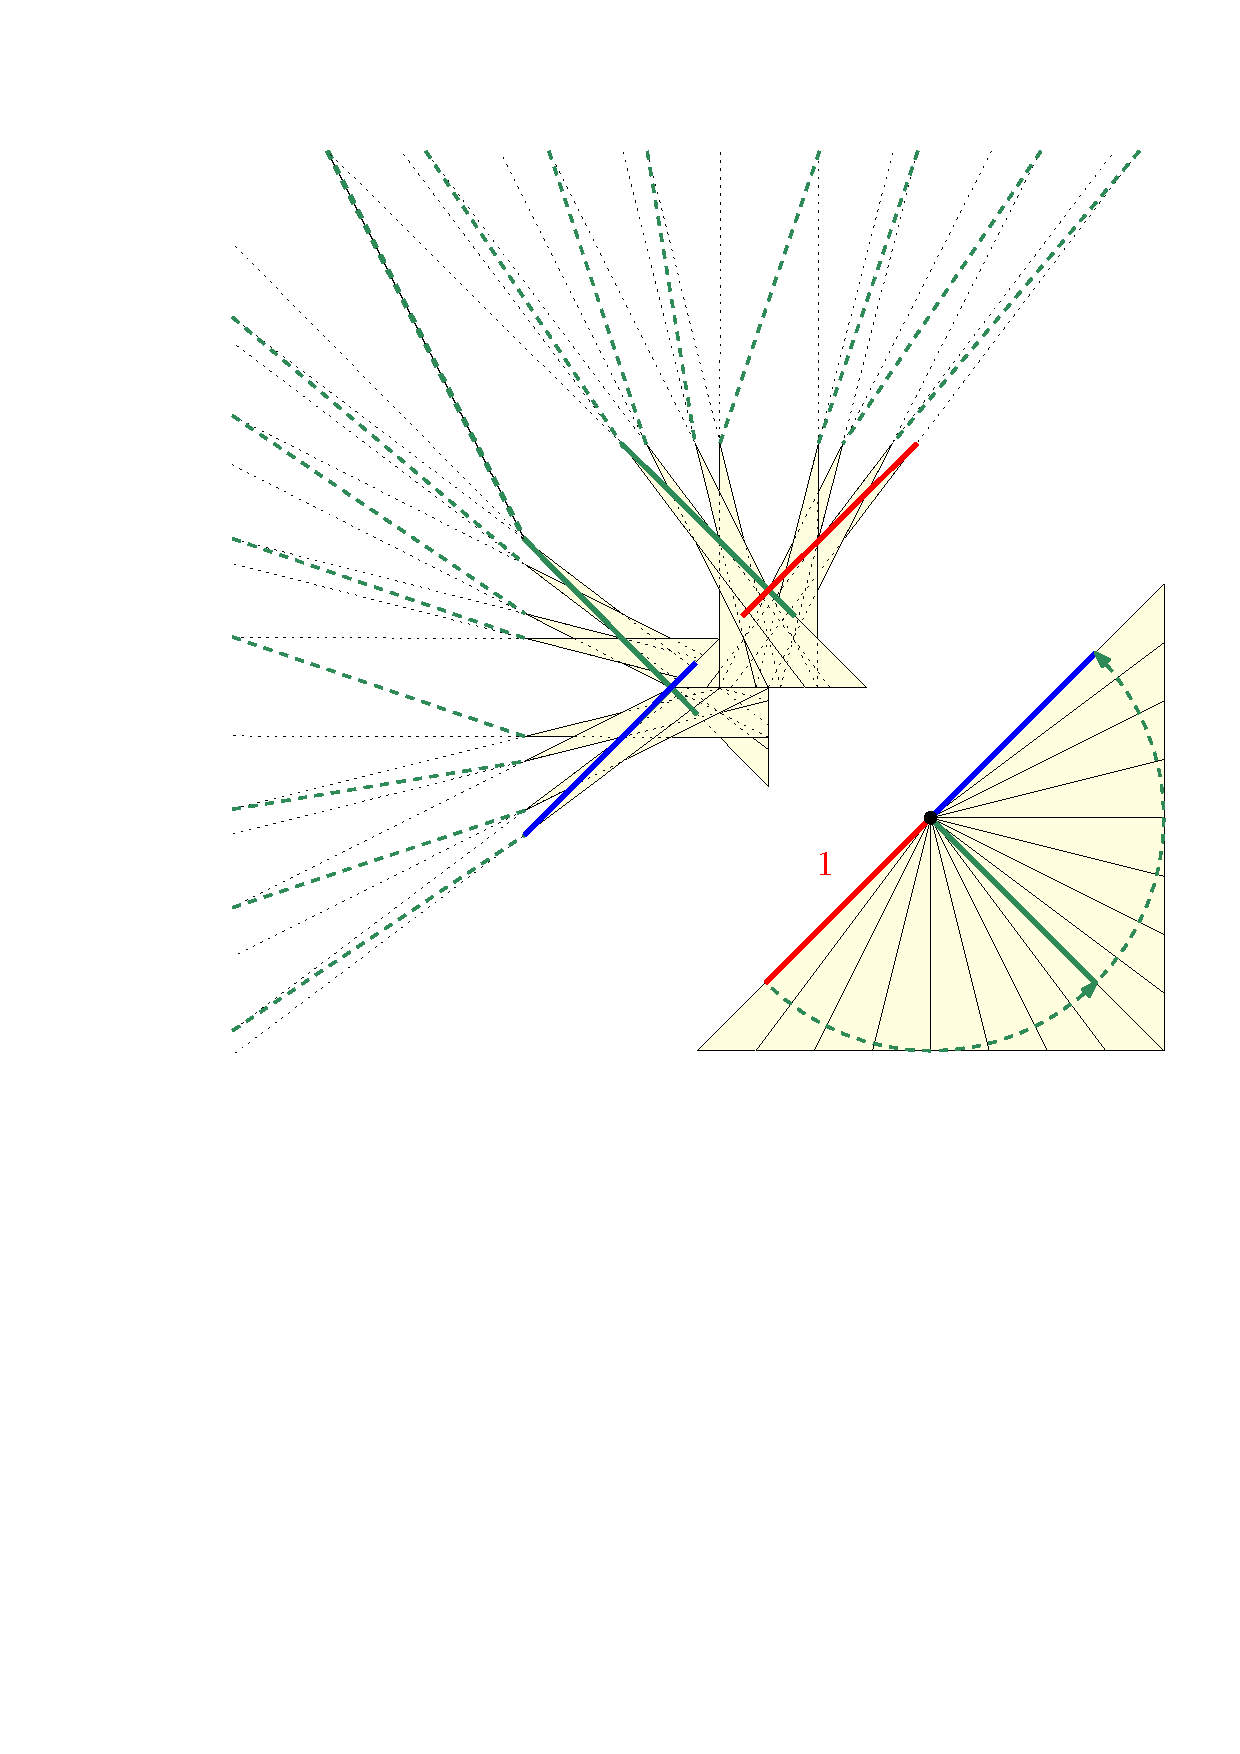
\includegraphics[width=0.9\textwidth]{ipe_slike/prehod_skupaj.pdf}
    \caption{Rotacija enotske daljice za 180° pri $ n = 8 $}
    \label{zdruzitev}
\end{figure}

Zaključimo z odgovorom na vprašanje Kakeye -- \textbf{ploščina območja, znotraj katerega se enotska daljica zvezno obrne za 360°, je lahko poljubno majhna}.

%%%%%%%%%%%%%%%%%%%%%%%%%%%%%%%%%%%%%%%%%%%%%%%%%%%%%%%%%%%%%%%%%
\section*{Zaključek}

Predstavljen je bil en način generiranja množice, ki ustreza pogovju iz vprašanja. Možnih konstrukcij je še več, vendar se v nadaljnje raziskovanje nisem spuščala. Omenim le še variacijo, kjer namesto pravokotnega enakokrakega trikotnika za osnovni trikotnik vzamemo enakostraničnega. V tem primeru je postopek brstenja dreves enak, le na koncu moramo namesto dveh skupaj ``zlepiti'' tri Perronova drevesa skupaj s spoji (slika~\ref{60_90}).

\begin{figure}[h!]
    \centering
    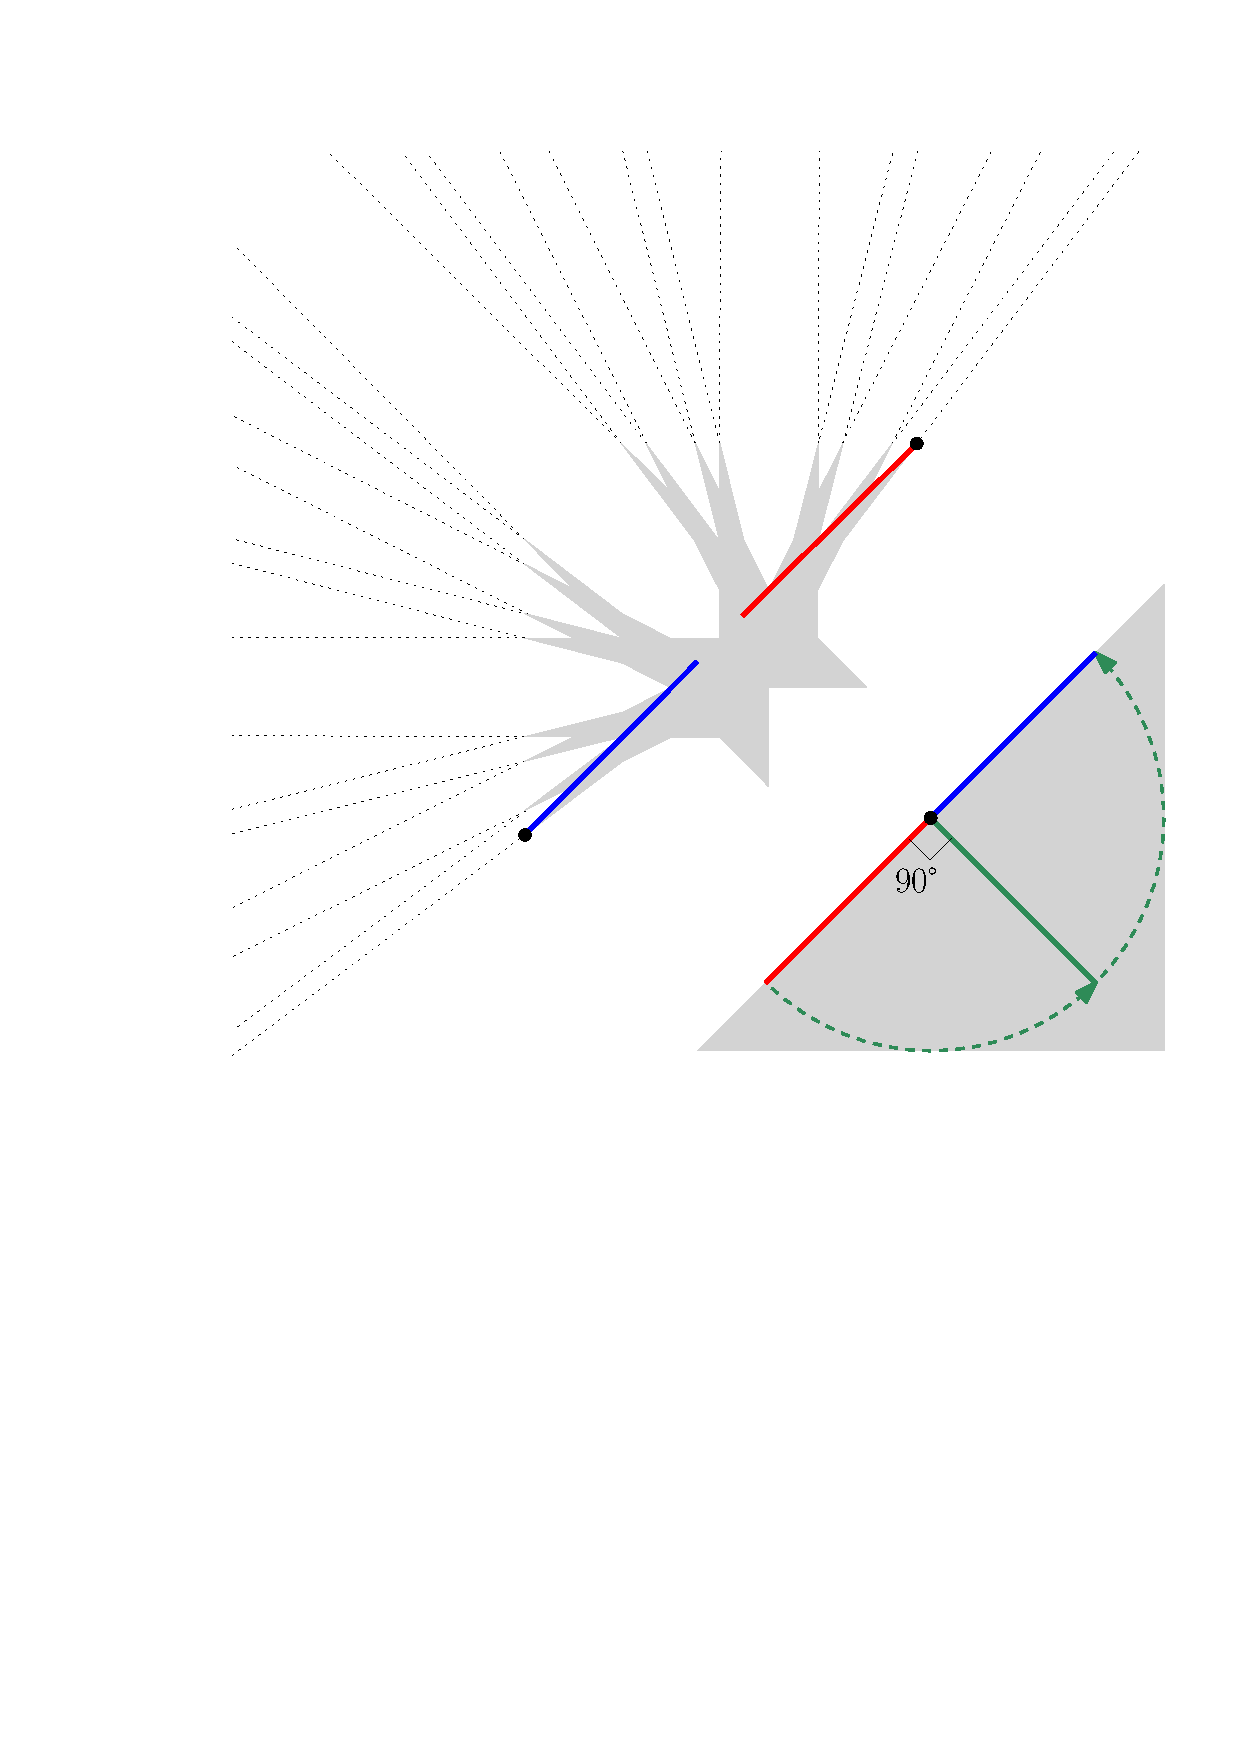
\includegraphics[width=0.45\textwidth]{ipe_slike/koncni_lik_90_napol_spoji.pdf}
    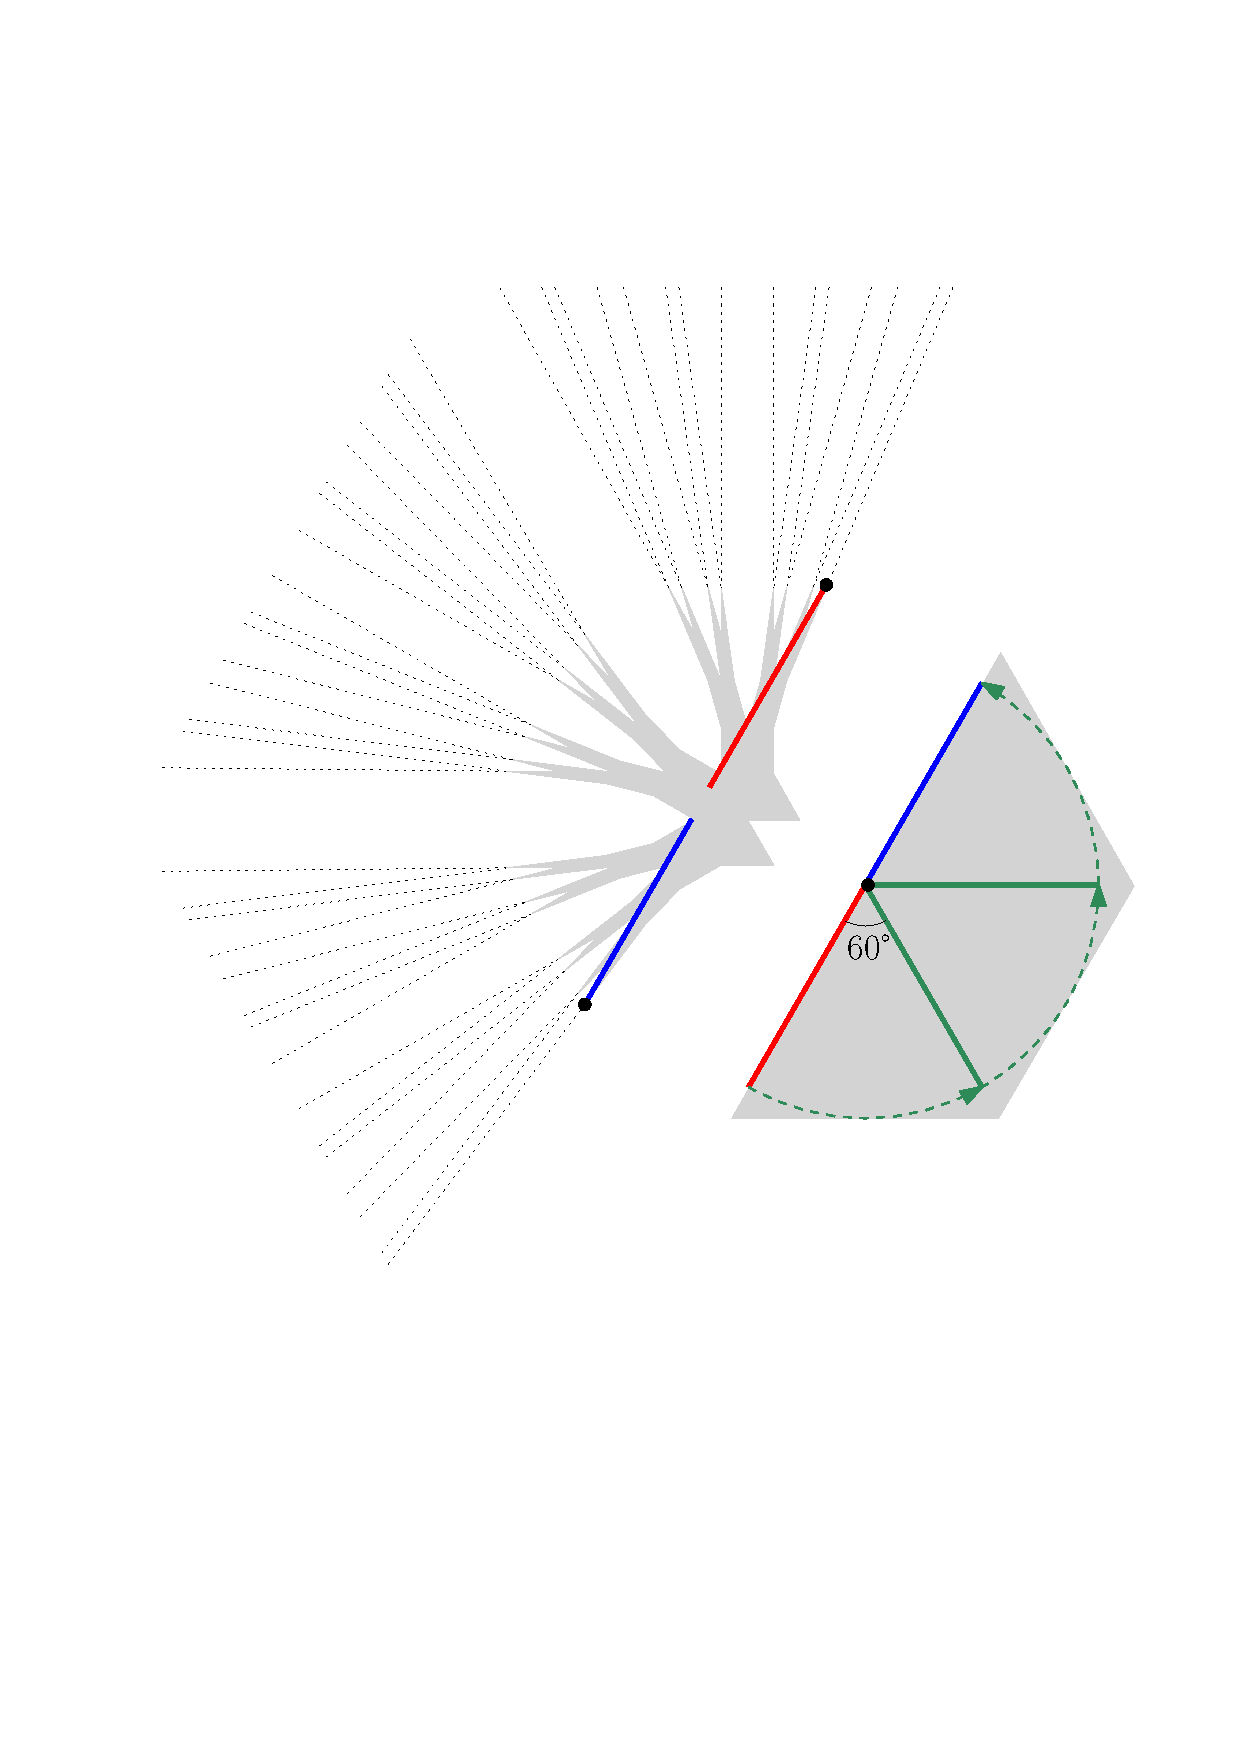
\includegraphics[width=0.45\textwidth]{ipe_slike/koncni_lik_60_napol_spoji.pdf}
    \caption{Primer spojenih Perronovih dreves pri dveh različnih osnovnih trikotnikih. Zaradi preglednosti so zelene povezave v spojih izpuščene}
    \label{60_90}
\end{figure}

Za nalogo sem imela vizualizacijo Kakeya-množice, ampak na začetku nisem vedela, kaj mora biti moj končni izdelek, zato sem se odločila za zapis članka s teoretično razlago ob večjem številu vizualnega gradiva za lažje razumevanje.

Osebno mi je tema naloge všeč, saj je bila zanimiva in hkrati ne pretežka, da je kakšni uspešnejši dijaki ne bi mogli razumeti. Ko sem poiskala malo več literature in posnetkov z animacijo (npr. \cite{YTNumberphile} in njegova preprostejša razlaga \cite{YTrazlaga}), sem lahko osnovni članek precej poenostavila in zapisala bolj razumljivo. Kar se tiče programa Ipe, sem nad njim zadovoljna, ker se marsikatero konstrukcijo z njim da hitreje narisati kot v Geogebri. Vendar ni njeno nadomestilo, saj ne zmore vizualizacije krivulj.

%%%%%%%%%%%%%%%%%%%%%%%%%%%%%%%%%%%%%%%%%%%%%%%%%%%%%%%%%%%%%%%%%
\newpage
\nocite{*}      % navede tudi vire, ki jih ne citiras
\printbibliography[heading=bibintoc, title={Literatura}]

%%%%%%%%%%%%%%%%%%%%%%%%%%%%%%%%%%%%%%%%%%%%%%%%%%%%%%%%%%%%%%%%%

\end{document}